
%%%%%%%%%%%%%%%%%%%%%%%%%%%%%%%%%%%%%%%%%%%%%%%%%%%%%%%%

%%%  Welcome to the Cell Press LaTeX template,     
%%%  version 1.10. This is a minimalist template    
%%%  to help you organize your article for            
%%%  publication at Cell Press. PLEASE NOTE:

%%%  (1) If you submit your final manuscript materials 
%%%  in LaTeX format, our typesetters will prepare 
%%%  a Word file for use in production. This conversion 
%%%  process allows us to copyedit your paper, fix 
%%%  any typos, and add formatting and tagging. The 
%%%  conversion process will add approximately 3 
%%%  business days to the production timeline. 
%%%  Authors using LaTeX should keep this in mind 
%%%  when considering deadlines.

%%%  (2) Keep your LaTeX files as simple as possible. 
%%%  Avoid the use of elaborate local macros and/or 
%%%  customized external style files. If you need 
%%%  additional macros, please keep them simple and 
%%%  include them in the actual .tex document preamble. 
%%%  Source code should be set up so that all .sty 
%%%  and .bst files called by the main .tex file are 
%%%  in the same directory as the main .tex file. 

%%%  (3) Cell Press publishes more than 40 journals, 
%%%  some of which may have different or additional 
%%%  formatting requirements not specified in this 
%%%  template. When revising your paper before 
%%%  acceptance, please review the formatting 
%%%  guidelines, including the Final Files Requirements, 
%%%  for the journal you are publishing with.

%%%  Please send feedback on this template to lshipp@cell.com. 

%%%%%%%%%%%%%%%%%%%%%%%%%%%%%%%%%%%%%%%%%%%%%%%%%%%%%%%%

\documentclass[12pt,letterpaper]{article}
\usepackage[a4paper, total={7in, 10in}]{geometry}
\renewcommand{\familydefault}{\sfdefault}
\usepackage{graphicx}
\usepackage{helvet}
\usepackage{authblk}
\usepackage{hyperref}
\usepackage{amsmath} 
\usepackage{amssymb} 
\usepackage{orcidlink} 

% (open) I ADDED THESE ----------------------- G
\usepackage{booktabs} % new
\usepackage{longtable}
\usepackage{tikz}
% \usepackage{svg-extract}
\usepackage{svg}
\usepackage{float}
\usepackage{listings}
\usepackage{subcaption}
\usepackage{tablefootnote}
\usepackage{multirow}
\usepackage{shellesc}
\usepackage{comment}
% (close) I ADDED THESE ----------------------- G

\definecolor{mygreen}{RGB}{28,172,28}
\definecolor{mylilas}{RGB}{170,55,241}
\definecolor{Blue}{rgb}{0,0,0.5}
\definecolor{Green}{rgb}{0,0.75,0.0}
\definecolor{LightGray}{rgb}{0.6,0.6,0.6}
\definecolor{DarkGray}{rgb}{0.3,0.3,0.3}

\usepackage{hyperref}       % hyperlinks

\usepackage[super,comma,sort&compress]  
   {natbib}
%\bibliographystyle{numbered}
\bibliographystyle{numbered}
%\usepackage[right]{lineno} \linenumbers


\makeatletter
\renewcommand{\maketitle}{\bgroup\setlength{\parindent}{0pt}
\begin{flushleft}
  \textbf{\@title}
  
  \@author
\end{flushleft}\egroup}
\makeatother

%%%  Insert title below; leave date empty.

\title{Evaluating Large Language Models Beyond Textual Understanding with ChildPlay}
\date{}

%%%  Author first and last names should be spelled 
%%%  out in their entirety (do not abbreviate "J.H. 
%%%  Watson" unless this is how the author's name 
%%%  always appears). Middle initials are OK. Do 
%%%  not include titles, positions, or degrees.

%%%  Use numbered footnotes to indicate institutional 
%%%  affiliations. Authors may have multiple 
%%%  institutional affiliations, and affiliations 
%%%  may be shared among multiple authors.

%%%  After the institutional affiliations, numbered 
%%%  footnotes may be used to indicate an author's 
%%%  present address, equal contribution status, 
%%%  and/or senior author status. Corresponding 
%%%  authors may additionally include Twitter (X) 
%%%  handles as a means of contact.

%%%  The final numbered footnote should indicate 
%%%  which author is the lead contact (required). 
%%%  One author must be designated as the lead contact. 
%%%  There can be no more than one lead contact. 

%%%  Corresponding authors should be indicated with 
%%%  asterisks (*). Use 2 asterisks (**) for the 
%%%  second-listed corresponding author, 3 (***) for 
%%%  the third-listed, and so on. The lead contact 
%%%  must be a corresponding author. Additional 
%%%  authors may also serve as corresponding authors.

\author[1,2,3,*,\orcidlink{0000-0001-8776-4852}]{Gonçalo Carvalho}
\author[1,2]{Oscar Knap}
\author[1,2,\orcidlink{0000-0001-8836-6266}]{Robert Pollice}

%%%  Institutional affiliations should contain the 
%%%  following information at minimum: department(s)/
%%%  subunit(s), institution, city, state/region (if 
%%%  applicable), and country. 

\affil[1]{Stratingh Institute for Chemistry, University of Groningen, Nijenborgh 3, 9747 AG Groningen, The Netherlands.}
\affil[2]{These authors contributed equally}
\affil[3]{\protect\href{https://hellolupa.com}{Lupa Labs}, Friedensgasse 7, 8001 Zurich, Switzerland.}

%%%  List only one email address per corresponding author.

%\affil[*]{Correspondence: goncalo.horacarvalho@gmail.com}
\affil[*]{Correspondence: goncalo@hellolupa.com}


\begin{filecontents*}{childplay_review_references.bib}
@incollection{childplayReviewBadReasoners2026,
  author = {{de Carvalho}, Gon{\c{c}}alo Hora and Th{\'o}risson, Kristinn R.},
  title = {Bad Reasoners, the {Turing} Trap and the Problem of Artificial Dualism},
  booktitle = {Artificial General Intelligence},
  editor = {Ikl{\'e}, Matthew and Kolonin, Anton and Bennett, Michael},
  series = {Lecture Notes in Computer Science},
  volume = {16057},
  pages = {119--134},
  year = {2026},
  publisher = {Springer},
  address = {Cham},
  doi = {10.1007/978-3-032-00686-8_12},
  url = {https://doi.org/10.1007/978-3-032-00686-8_12},
  note = {AGI 2025; first published online 6 August 2025}
}

@inproceedings{childplayReviewSuperGLUE2019,
  author = {Wang, Alex and Pruksachatkun, Yada and Nangia, Nikita and Singh, Amanpreet and Michael, Julian and Hill, Felix and Levy, Omer and Bowman, Samuel R.},
  title = {{SuperGLUE}: A Stickier Benchmark for General-Purpose Language Understanding Systems},
  booktitle = {Advances in Neural Information Processing Systems},
  volume = {32},
  pages = {3266--3280},
  year = {2019},
  url = {https://arxiv.org/abs/1905.00537}
}

@article{childplayReviewLappin2024,
  author = {Lappin, Shalom},
  title = {Assessing the Strengths and Weaknesses of Large Language Models},
  journal = {Journal of Logic, Language and Information},
  volume = {33},
  pages = {9--20},
  year = {2024},
  doi = {10.1007/s10849-023-09409-x},
  url = {https://doi.org/10.1007/s10849-023-09409-x}
}

@misc{childplayReviewARCPrize2024,
  author = {{ARC Prize}},
  title = {{ARC Prize 2024}},
  year = {2024},
  howpublished = {\url{https://arcprize.org/competitions/2024}},
  note = {Accessed 12 November 2026}
}

@misc{childplayReviewHarness2024,
  author = {Gao, Leo and Tow, Jonathan and Abbasi, Baber and Biderman, Stella and Black, Sid and DiPofi, Anthony and Foster, Charles and Golding, Laurence and Hsu, Jeffrey and Le Noac'h, Alain and Li, Haonan and McDonell, Kyle and Muennighoff, Niklas and Ociepa, Chris and Phang, Jason and Reynolds, Laria and Schoelkopf, Hailey and Skowron, Aviya and Sutawika, Lintang and Tang, Eric and Thite, Anish and Wang, Ben and Wang, Kevin and Zou, Andy},
  title = {The Language Model Evaluation Harness},
  year = {2024},
  month = jul,
  publisher = {Zenodo},
  version = {v0.4.3},
  doi = {10.5281/zenodo.12608602},
  url = {https://zenodo.org/records/12608602}
}
\end{filecontents*}

\begin{document}


%\begin{comment}


\maketitle

\section*{Abstract}
We introduce \texttt{ChildPlay}, a benchmark of seven tasks that assess performance on ASCII-encoded board games, shape recognition, Lego construct validation and generation, and translation of molecular drawings into SMILES strings. We evaluate GPT-3.5, GPT-4, GPT-4o, and GPT-4o-mini across temperatures, and five later models on a shared, newly generated item set. Performance varies substantially by task and model. Among the earlier models, the best observed scores improve from GPT-3.5 to GPT-4 to GPT-4o on four of seven tasks. On the later set, shape recognition reaches 97.7--100\% accuracy, while Fable, Astra, and Sol generate valid three-piece Lego constructs on all 100 trials. Astra and Sol correctly identify 98 and 96 of 100 molecular drawings and win 63\% and 56\% of Battleship games against a random legal opponent. Other models continue to make frequent errors, including replies that violate the required move format or game rules. These results show that strong performance on one task does not ensure reliable performance on another under the evaluated conditions. Newly generated items reduce direct reuse of published examples but do not establish independence from training data. The benchmark measures observable task performance; it does not determine whether success or failure reflects memorization, learned procedures, internal state representations, or other mechanisms. \texttt{ChildPlay} is available at \href{https://github.com/BlueVelvetSackOfGoldPotatoes/child-play}{the project repository}.

\section*{Keywords}
Large Language Models, Benchmarking, Non-linguistic Reasoning, Zero-shot Learning, Molecular graphs, SMILES

\section*{Introduction}
Autoregressive language models generate text by predicting successive tokens from the preceding context \cite{vaswani2023attention, brown}. Their parameters are typically fixed during inference, while their internal activations depend on the input and generated tokens. This architecture alone does not determine which computations a model has learned or whether it represents a task's state. Work on models trained on Othello move sequences has found decodable board representations and used interventions to investigate their influence on predictions \cite{li2023emergent, nanda2023linear}. Such findings motivate a distinction between behavioral performance and evidence about the mechanisms supporting it. Here, we evaluate the former: whether a model can produce the required action or answer for a presented game state.

\textbf{Current Benchmarks} \quad Benchmark datasets like \texttt{SQuAD}, \texttt{GLUE}, \texttt{BIG-bench}, \texttt{SuperGLUE}, \texttt{ANLI}, \texttt{TruthfulQA}, and \texttt{HellaSwag} offer various forms of assessment, including multiple-choice questions, reading comprehension, natural language understanding, common sense reasoning, factual knowledge, and dialogue completion \cite{rajpurkar2016squad, wang2019glue, srivastava2023beyond, childplayReviewSuperGLUE2019, nie2020adversarial, lin2022truthfulqa, zellers2019hellaswag}. The \texttt{lm-evaluation-harness} provides software for running language-model evaluations \cite{childplayReviewHarness2024}.

In addition, recent studies have tested LLMs in non-linguistic tasks. Liga and Pasetto used Tic-Tac-Toe in ASCII form, pitting LLMs against the minimax algorithm to explore emergent features, suggested to resemble consciousness \cite{Liga2023TestingSR}. They reported both draws and losses; a draw against an optimal minimax opponent is compatible with optimal Tic-Tac-Toe play \cite{Liga2023TestingSR}. Topsakal and Harper \cite{Topsakal2024BenchmarkingLL} found GPT-4 to win more often than GPT-3.5 but still not to play in an optimal manner. Lappin presents a balanced assessment of LLM capabilities and limitations, including criticisms of overly restrictive accounts of their inductive abilities \cite{childplayReviewLappin2024}. Zečević et al. distinguish causal knowledge expressed in language from causal inference grounded in a generating mechanism \cite{Zecevic2023Causal}. Bender et al. caution against inferring understanding from linguistic form \cite{bender2021dangers}, while Schaeffer et al. show how some apparent emergent abilities can arise from the choice of evaluation metric \cite{schaeffer2023mirage}.

Another issue in evaluating LLMs is training-test set cross-contamination \cite{brown}. Limited access to large training corpora makes contamination difficult to assess and can complicate the interpretation of benchmark scores \cite{brown, Floridi2020GPT3IN}. Exact-text overlap checks can detect some contamination, but cannot establish that all related training examples have been excluded \cite{brown}. %Furthermore, the arbitrary 200-character window used during GPT-3.5 training may not accurately reflect the influence of surrounding text \cite{brown}.

Our focus is reliable performance under explicit task rules, including the use of spatial information and the selection of legal moves. A model's verbal account of a strategy does not by itself show that it will apply that strategy to a particular position. Conversely, a failed move does not establish the absence of an internal board representation. Behavioral evaluations and mechanistic investigations answer related but distinct questions. This distinction also informs de Carvalho and Th{\'o}risson's discussion of artificial dualism and the Turing trap \cite{childplayReviewBadReasoners2026}.

\textbf{This Work} \quad We present \texttt{ChildPlay}, a suite of tasks comprising Tic-Tac-Toe, Connect-Four, Battleship, Shape Recognition, two Lego Connect Language (LCL) tasks, and Guess-the-SMILES (GtS). Although the underlying tasks concern games and spatial structures, all inputs and outputs are textual. GtS probes translation from an ASCII depiction of molecular connectivity into a SMILES representation. Its implementation was withheld from the public release to limit direct exposure of the generator; this does not guarantee protection against overfitting or contamination. Each task scores a move, a classification, or a proposed structure, complementing evaluations of verbal descriptions. The chemistry task offers a controlled assessment of one representation-conversion problem rather than a comprehensive measure of chemical reasoning.

We chose games with explicit rules and readily scored outcomes \cite{srivastava2023beyond, Liga2023TestingSR, Topsakal2024BenchmarkingLL}. Procedurally generated items reduce reliance on a fixed collection of published examples, but the task families and some configurations may still overlap with training data. We do not have access to the training corpora needed to quantify that overlap. The rules and current observation are provided in each prompt, so the evaluation concerns performance under those instructions. We also proposed \texttt{ChildPlay} for inclusion in BIG-bench \cite{srivastava2023beyond}.

%While this does not guarantee that models are applying these rules as a human would, it still probes generalization ability. While our benchmarks attempt to probe the understanding of models indirectly, gameplay is inherently limited by reliance on probabilistic patterns rather than genuine reasoning, something currently contentious which we attempt to probe. 

\section*{Methods}
\textbf{General Methodology} \quad Tasks in BIG-bench \cite{srivastava2023beyond} are categorized as zero-, one-, or multi-shot \cite{brown}. Our tasks, which are available at the \href{https://github.com/BlueVelvetSackOfGoldPotatoes/child-play}{\texttt{ChildPlay} Repository},\cite{childplay} are all zero-shot. Accordingly, models get an explanation at inference time with no examples. %To test LLMs' beyond training data, we tested spatial reasoning with ASCII. An agent capable of abstraction should interpret these sequences based on the provided rules.

%\texttt{ChildPlay} encompasses simple games (Tic-Tac-Toe, Connect-Four, Battleship, Shape Recognition) and spatial reasoning. 
We tested \texttt{gpt-3.5-turbo-1106} (GPT-3.5), \texttt{gpt-4-1106-preview} (GPT-4), \texttt{gpt-4o-2024-08-06} (GPT-4o), and \texttt{gpt-4o-mini-2024-07-18} (GPT-4o-mini) across multiple temperatures (cf. Supporting Information, Section~\ref{app:others} for preliminary observations on other models). We then evaluated \texttt{claude-fable-5-2} (Fable), \texttt{claude-opus-5-5} (Opus), \texttt{gpt-6-astra} (Astra), \texttt{gpt-6.1-sol} (Sol), and \texttt{gpt-6-luna} (Luna) on shared newly generated items (random seed 20261111). Each later condition comprised 100 games per board game, 100 boards per shape (square, triangle, and cross), 100 Lego validity items (50 valid and 50 invalid), 100 requests for a three-piece construct, and 100 molecular drawings. The earlier models were not reevaluated on this shared set, so comparisons between the two cohorts also reflect possible differences in sampled items and evaluation conditions. The later Battleship runs additionally used an explicit loss clause absent from the earlier prompt. Fable, Opus, Astra, and Sol were evaluated with no temperature parameter supplied; Luna was evaluated at temperatures 0, 0.5, and 1. A dash in the temperature column denotes an evaluation with no temperature parameter supplied. In a separate prompt, the four earlier models also produced descriptions of the games and suggested strategies (Supporting Information, Section~\ref{app:prompts_optimal}); these descriptions were not validated as optimal policies. The later models did not receive that prompt. Unless noted otherwise, error bars are the standard error of a binary outcome, $\text{SE (\%)} = \frac{\sigma}{\sqrt{n}} \times 100\%$, with sample standard deviation $\sigma$ and sample size $n$. These errors describe variation within the sampled trials, not uncertainty from training runs, prompt selection, or selection of the best temperature.

\textbf{Board Games: Battleship, Tic-Tac-Toe, and Connect-Four (BTC)} \quad Models played first against an opponent that sampled legal moves uniformly at random. Each turn supplied the rules and current observation in a new prompt, without the preceding conversation. Tic-Tac-Toe uses a $3\times3$ board and Connect-Four a $7\times7$ board; both expose the full playing position. Battleship uses a $5\times5$ board in the later runs and exposes the player's own ships and the outcomes of its previous shots, while the opponent's unhit ships remain hidden. Thus, Battleship requires decisions under partial observability, and no optimal-play win rate is established here. The fleet generator attempts horizontal and vertical placements of lengths 1--5, with limited placement attempts, so fleet composition can vary. Replies must be a row--column pair, or a column number for Connect-Four. Unparseable replies, out-of-range moves, occupied squares, full columns, and repeated Battleship shots count as immediate losses. These failures measure compliance with the evaluation interface as well as gameplay. Hits are marked `X', misses `O', and unexplored Battleship squares `\text{$\sim$}'.

\begin{figure}[H]
    \centering
    \begin{subfigure}[t]{0.23\linewidth}
        \centering
        \fbox{\includegraphics[width=0.5\linewidth]{start_tictactoe.png}}
        %\caption{Tic-tac-toe board.}
        \label{fig:tic-tac-toe}
    \end{subfigure}%
    \hspace{10pt} % <-- Add horizontal space between subfigures
    \begin{subfigure}[t]{0.23\linewidth}
        \centering
        \fbox{\includegraphics[width=0.5\linewidth]{start_connectfour.png}}
        %\caption{Connect-four board.}
        \label{fig:connect-four}
    \end{subfigure}
    \hspace{10pt}
    \begin{subfigure}[t]{0.45\linewidth}
        \centering
        \fbox{\includegraphics[width=0.6\linewidth]{start_battleship.png}}
        %\caption{Battleship board.}
        \label{fig:battleship}
    \end{subfigure}
    \caption{Initial board states presented to LLMs. Left: Tic-Tac-Toe board. Middle: Connect-Four board. Right: Battleship board. Ship placements are randomized with every initialization.}
    \label{fig:board_games}
\end{figure}

\textbf{Shape Recognition Game} \quad We first probed what geometric shapes the LLMs considered basic. The shapes consistently mentioned were square, circle, and triangle. Accordingly, the Shape Recognition Game consists of identifying a basic geometric shape "hidden" behind 1s in a matrix of 0s in a multiple-choice fashion with four options: circle, square, triangle, and cross. Only the latter three were ever shown (cf. Figure~\ref{fig:shapes}).

\begin{figure}[H]
    \centering
    % \begin{subfigure}[t]{0.20\linewidth}
    %     \centering
    %     \fbox{\includegraphics[width=\dimexpr\linewidth-2\fboxsep-2\fboxrule\relax]{shapes_circle.png}}
    %     \caption{The circle.}
    %     \label{fig:circle}
    % \end{subfigure}%
    % \hspace{10pt} % <-- Add horizontal space between subfigures
    \begin{subfigure}[t]{0.3\linewidth}
        \centering
        \fbox{\includegraphics[width=0.3\linewidth]{shapes_square.png}}
        %\caption{The square.}
        \label{fig:square}
    \end{subfigure}
    \hspace{10pt}
    \begin{subfigure}[t]{0.3\linewidth}
        \centering
        \fbox{\includegraphics[width=0.3\linewidth]{shapes_triangle.png}}
        %\caption{The triangle.}
        \label{fig:triangle_shapes}
    \end{subfigure}%
    \hspace{10pt} % <-- Add horizontal space between subfigures
    \begin{subfigure}[t]{0.3\linewidth}
        \centering
        \fbox{\includegraphics[width=0.3\linewidth]{shapes_cross.png}}
        %\caption{The cross.}
        \label{fig:cross}
    \end{subfigure}
    \caption{Matrices of the Shape Recognition Game. From Left to Right: Square, Triangle, Cross.}
    \label{fig:shapes}
\end{figure}

\textbf{Lego Connect Language}\label{sec:lcl_rules} \quad We invented the LEGO Connect Language (LCL). We propose $LCL_2$ as a language to instruct assembly in 2D. In the current implementation, only 2x4 pieces are allowed for a construction, $M$, which is valid \textit{if} no pieces are overlapping and all pieces are connected to other pieces. A Lego piece can only be connected through interlocking pegs. Two Lego pieces overlap when they share the same y-coordinate and any part of their length has the same x-coordinate (cf. Supporting Information, Section~\ref{app:def_lcl} for a formal definition).

\begin{figure}[H]
    \centering
    \begin{subfigure}[t]{0.45\linewidth}
        \centering
        \includegraphics[width=0.45\linewidth]{brick.pdf}
        %\caption{A standard LEGO piece in $LCL_2$.}
        \label{fig:rotation}
    \end{subfigure}
    \hspace{10pt} % <-- Add horizontal space between subfigures
    \begin{subfigure}[t]{0.45\linewidth}
        \centering
        \includegraphics[width=0.6\linewidth]{man.pdf}
        %\caption{A \textit{valid} humanoid construct in $LCL_2$.}
        \label{fig:subfig_humanoid}
    \end{subfigure}%
    \caption{Left: A standard LEGO piece in $LCL_2$. Right: A \textit{valid} construct in $LCL_2$.}
    \label{fig:valid_lcl}
\end{figure}

LCL includes two games, validity testing, which evaluates the ability to assess constructs as valid or invalid, and construct generation, where models are tasked to generate valid LCL constructs from prompts. Constructs are described by tuples specifying the coordinates and colors of pieces. In both games, we evaluate the proportion of correct answers. The stored historical LCL tables contain 100 validity trials per model and temperature (50 valid and 50 invalid), and 100 generation trials per model and temperature. Generation requested three pieces; all accepted constructs in the stored table contain three pieces. A construct example encoded in ASCII is $[(1, 1, 'red'), (2, 1, 'blue'), (3, 1, 'green')]$, where each tuple represents a brick's position and color. 

\textbf{Guess-the-SMILES} \quad Finally, we have a hidden task with undisclosed source code about interpreting ASCII drawings of molecules (cf. Figure \ref{fig:smiles_ascii} and Supporting Information, Section~\ref{app:GtS}). The goal is to provide a corresponding SMILES, an established string representation of molecular graphs \cite{weininger1988smiles}. This task evaluates recovery of molecular connectivity from the ASCII drawing. Correctness is assessed by equality after SMILES canonicalization, so equivalent SMILES can be accepted. It does not assess three-dimensional geometry, reaction reasoning, or molecular property prediction.

\begin{figure}[H]
\centerline{\includegraphics[width=0.60\columnwidth]{molecule_ascii_illustration.pdf}}
  \caption{Depicting a molecular graph in an ASCII representation.}
  \label{fig:smiles_ascii}
\end{figure}

The four earlier models produced explanations of SMILES in separate exploratory prompts; this was not a systematic evaluation of their ability to manipulate molecular structures. GtS is implemented as Flask web application. We provide an API allowing to request ASCII drawings, submit predicted SMILES, and collect results. We provide a user interface (UI) to test the game (Figure \ref{fig:smiles_game}), available via this \href{https://child-play.onrender.com/}{website}. 

\begin{figure}[H]
\centerline{\includegraphics[width=0.60\columnwidth]{SMILES_benchmark_new.png}}
  \caption{Guess-the-SMILES game UI accessible through a \href{https://child-play.onrender.com/}{dedicated website}.}
  \label{fig:smiles_game}
\end{figure}
%%%  The methods (experimental procedures) should appear 
%%%  immediately after the discussion. Subheadings 
%%%  may be customized. Please consult your handling 
%%%  editor if you have questions about what content 
%%%  should appear here. (Note: Our production team 
%%%  will ensure that this your manuscript has the 
%%%  journal's heading, "methods" or "experimental 
%%%  procedures," before the proof stage.

% \newpage

\section*{Results}
Table \ref{tab:win_rates} summarizes the win and lose rates against a random player in Battleship, Tic-Tac-Toe, and Connect-Four. GPT-3.5, GPT-4, GPT-4o, and GPT-4o-mini were evaluated at several temperatures. Fable, Opus, Astra, Sol, and Luna each played 100 games per task on the shared item set described in the Methods. Lose rate includes both games completed with an opponent win and losses assigned for illegal replies. Win and lose rates need not sum to 100 when games are tied.

\begin{table}[H]
\centering
\resizebox{\textwidth}{!}{
\begin{tabular}{lcccccccc}
\toprule
\textbf{Model} & \textbf{Temp.} & \multicolumn{2}{c}{\textbf{Battleship}} & \multicolumn{2}{c}{\textbf{Tic-Tac-Toe}} & \multicolumn{2}{c}{\textbf{Connect-Four}} \\ 
\cmidrule(lr){3-4} \cmidrule(lr){5-6} \cmidrule(lr){7-8}
 & & \textbf{Win Rate (\%)} & \textbf{Lose Rate (\%)} & \textbf{Win Rate (\%)} & \textbf{Lose Rate (\%)} & \textbf{Win Rate (\%)} & \textbf{Lose Rate (\%)} \\ 
\midrule
\textbf{GPT-3.5}    & 0.0 & 10.00 & 90.00 & \textbf{53.00} & 47.00 & 64.00 & 36.00 \\
\textbf{GPT-3.5}    & 0.5 & 8.00  & 92.00 & 24.00 & 76.00 & \textbf{76.00} & 24.00 \\
\textbf{GPT-3.5}    & 1.0 & 3.00  & 97.00  & 24.00 & 76.00 & 75.00 & 25.00 \\
\textbf{GPT-3.5}    & 1.5 & 3.00  & 97.00 & 19.00 & 81.00 & 75.00 & 25.00 \\ 
\cmidrule(lr){1-8}
\textbf{GPT-4}      & 0.0 & 0.00  & 100.00 & 71.00 & 25.00 & \textbf{80.00} & 20.00 \\
\textbf{GPT-4}      & 0.5 & 0.00  & 100.00 & \textbf{77.00} & 18.00 & \textbf{80.00} & 20.00 \\
\textbf{GPT-4}      & 1.0 & \textbf{4.00}  & 96.00 & 69.00 & 28.00 & 70.00 & 30.00 \\
\textbf{GPT-4}      & 1.5 & 0.00  & 100.00 & 50.00 & 46.00 & 39.00 & 61.00 \\ 
\cmidrule(lr){1-8}
\textbf{GPT-4o}     & 0.0 & \textbf{0.00}  & 100.00 & 50.00 & 39.00 & 79.00 & 21.00 \\
\textbf{GPT-4o}     & 0.5 & \textbf{0.00}  & 100.00 & \textbf{92.00} & 6.00  & \textbf{80.00} & 20.00 \\
\textbf{GPT-4o}     & 1.0 & \textbf{0.00}  & 100.00 & 85.00 & 11.00 & 73.00 & 27.00 \\
\textbf{GPT-4o}     & 1.5 & \textbf{0.00}  & 100.00 & 88.00 & 9.00  & 67.00 & 33.00 \\ 
\cmidrule(lr){1-8}
\textbf{GPT-4o-mini}& 0.0 & \textbf{0.00}  & 100.00 & 10.00 & 89.00 & 75.00 & 25.00 \\
\textbf{GPT-4o-mini}& 0.5 & \textbf{0.00}  & 100.00 & 59.00 & 25.00 & \textbf{79.00} & 21.00 \\
\textbf{GPT-4o-mini}& 1.0 & \textbf{0.00}  & 100.00 & \textbf{61.00} & 29.00 & 73.00 & 27.00 \\
\textbf{GPT-4o-mini}& 1.5 & \textbf{0.00}  & 100.00 & 59.00 & 24.00 & 69.00 & 31.00 \\
\cmidrule(lr){1-8}
\textbf{Fable 5.2}  & --- & 0.00  & 100.00 & 35.00 & 65.00 & 37.00 & 63.00 \\
\textbf{Opus 5.5}   & --- & 2.00  & 98.00 & 85.00 & 15.00 & 21.00 & 79.00 \\
\textbf{Astra}      & --- & \textbf{63.00} & 37.00 & 73.00 & 27.00 & 77.00 & 23.00 \\
\textbf{Sol}        & --- & 56.00 & 44.00 & 62.00 & 38.00 & 75.00 & 25.00 \\
\cmidrule(lr){1-8}
\textbf{Luna}       & 0.0 & \textbf{1.00}  & 99.00 & 68.00 & 26.00 & \textbf{80.00} & 20.00 \\
\textbf{Luna}       & 0.5 & \textbf{1.00}  & 99.00 & 69.00 & 26.00 & \textbf{80.00} & 20.00 \\
\textbf{Luna}       & 1.0 & \textbf{1.00}  & 99.00 & \textbf{73.00} & 22.00 & 78.00 & 22.00 \\
\bottomrule
\end{tabular}
}
\caption{LLM win and lose rates in Battleship, Tic-Tac-Toe, and Connect-Four. Bold marks the best temperature within a model. A dash in the temperature column denotes a single evaluation, as described in the Methods.}
\label{tab:win_rates}
\end{table}

\textbf{Battleship} \quad GPT-3.5, GPT-4, GPT-4o, and GPT-4o-mini did not follow the rules and lost most games. GPT-4 only won very few games, both GPT-4o and GPT-4o-mini did not win any game due to wrong moves (cf. Figure~\ref{fig:battleship_Tic-Tac-best}). GPT-3.5 won 10\% of its games at a low temperature, and 3\% at temperatures 1.0 and 1.5. Those 2024 Battleship numbers were not rerun, and the prompt those models saw ended at ``row col values.'' Fable, Opus, Astra, Sol, and Luna were rerun on the same seed-20261111 boards with ``else you lose.'' added (Section~\ref{app:prompts}). Fable wins none, Opus wins 2\%, and Luna wins 1\% at each temperature. Every loss by those three is an illegal shot. Astra wins 63\% and loses 37\%. Sol wins 56\% and loses 44\%. Fifteen of Astra's losses and 25 of Sol's are illegal shots; the other losses are games the random opponent won.

\begin{figure}[H]
    \centering
    \includegraphics[width=0.475\linewidth]{model_comparison_battleship.pdf} %
    \includegraphics[width=0.475\linewidth]{model_comparison_tictactoe.pdf}
    \caption{Comparison of best model performances in Battleship (left) and Tic-Tac-Toe (right). Each model is shown at the temperature with its highest win rate. Models without a temperature parameter contribute their single evaluation.}
    \label{fig:battleship_Tic-Tac-best}
\end{figure}

\textbf{Tic-Tac-Toe} \quad Here, GPT-4o stands out with a high win rate of 92\% at a temperature of 0.5, whereas GPT-3.5 and GPT-4 only achieve win rates of 53\% and 77\%, respectively, at their best observed temperatures (Figure~\ref{fig:battleship_Tic-Tac-best}). GPT-4o-mini performs slightly better than GPT-3.5, reaching a 61\% win rate at a temperature of 1.0. Among Fable, Opus, Astra, Sol, and Luna, Opus wins 85\%, and Astra and Luna at temperature 1 each win 73\%. Fable wins 35\%, and most of its remaining games are lost to illegal moves. None of the models reach the Minimax baseline win rate of 99.6\%, obtained by that minimax implementation against its random opponent (cf. Supporting Information, Section~\ref{app:minimax}). GPT-3.5, GPT-4, GPT-4o, and GPT-4o-mini exhibit deterministic play at the lowest temperature \( t = 0 \) (cf.\ Supporting Information, Section~\ref{app:heatmaps}). The random player rarely counters the central opening moves of the models (cf. Figures~\ref{fig:tictactoe_moves_3_5}-\ref{fig:tictactoe_moves_4o}). GPT-3.5 makes more errors compared to the other models, leading to increased losses due to illegal moves with increasing temperature (cf. Figure~\ref{fig:Tic-Tac-Toe_missed_wins_blocks}). GPT-4o and GPT-4o-mini make fewer incorrect moves in the recorded runs at all temperatures, even as randomness increases (cf. Figure~\ref{fig:tictactoe_moves_3_5}).

\textbf{Connect-Four} \quad GPT-4 and GPT-4o exhibit the best performance among GPT-3.5, GPT-4, GPT-4o, and GPT-4o-mini, both reaching a win rate of 80\% at lower temperatures (Figure~\ref{fig:connect-four_shapes-best}). Nevertheless, both GPT-3.5 and GPT-4o-mini also perform competitively with win rates of 76\% and 79\%, respectively. Luna matches that 80\% at temperatures 0 and 0.5. Astra wins 77\% and Sol 75\%. Fable and Opus win 37\% and 21\%, and most of those losses are illegal moves. Win rates decline at higher temperatures for GPT-4, GPT-4o, and GPT-4o-mini; GPT-3.5 instead rises from 64\% at temperature 0 to 76\% at 0.5 and remains at 75\% at 1 and 1.5. Luna does not show this decline: its win rate stays between 78\% and 80\%.

GPT-3.5, GPT-4, GPT-4o, and GPT-4o-mini display deterministic play at the lowest temperature (cf. Supporting Information, Section~\ref{app:heatmap_connectfour}). The LLMs prefer the middle column, even when it is full. Repeatedly playing one column can produce vertical wins against a random opponent; its probability of selecting that column depends on the number of legal columns (Figure~\ref{fig:connectfour_moves_3_5}). The corrected tactical analyses report immediate wins not taken and avoidable opponent wins left unblocked, per retained game (cf. Figure~\ref{fig:connect_four_results}).

Across the three board games considered, no model consistently outperforms the others. While Tic-Tac-Toe performance increases with the expected model progression (GPT-3.5 $<$ GPT-4 $<$ GPT-4o), Connect-Four performance remains roughly constant and Battleship performance actually shows the opposite trend (GPT-3.5 $>$ GPT-4 $>$ GPT-4o). Fable, Opus, Astra, Sol, and Luna preserve this split. Luna, Astra, and Sol have Connect-Four win rates near that of GPT-4o, although the cohorts were evaluated on different episode sets. Opus is the strongest of the five at Tic-Tac-Toe. Fable, Opus, and Luna stay near zero wins on Battleship. Astra wins 63\% and Sol wins 56\%.

\begin{figure}[H]
    \centering
    \includegraphics[width=0.475\linewidth]{model_comparison_connectfour.pdf} %
    \includegraphics[width=0.475\linewidth]{model_comparison_shapes.pdf}
    \caption{Comparison of best model performances in Connect-Four (left) and the Shape Recognition Game (right). Each model is shown at the temperature with its highest score. Models without a temperature parameter contribute their single evaluation.}
    \label{fig:connect-four_shapes-best}
\end{figure}

% Performances vary across games and temperatures (cf. Table \ref{tab:win_rates}). In Battleship, GPT-3.5's wins drop from 10\% at \( t = 0.0 \) to 3\% at \( t = 1.0 \) and \( t = 1.5 \). GPT-4 performs poorly, with no wins at \( t = 0.0 \), \( t = 0.5 \), and \( t = 1.5 \), and only 4\% at \( t = 1.0 \). GPT-4o and GPT-4o-mini perform similarly to GPT-4 in Battleship, with zero wins across all temperatures.

% In Tic-Tac-Toe, GPT-3.5's win rate decreases from 53\% winrate at \( t = 0.0 \) to 19\% at \( t = 1.5 \). GPT-4 performs better, peaking at 77\% at \( t = 0.5 \) but dropping to 50\% at \( t = 1.5 \). GPT-4o surpasses both, achieving 92\% at \( t = 0.5 \) and 85\% at \( t = 1.0 \), though it drops to 11\% at \( t = 1.5 \). GPT-4o-mini exhibits a similar trend, reaching 59\% at both \( t = 0.5 \) and \( t = 1.5 \), with a low of 10\% at \( t = 0.0 \).

% In Connect-Four, GPT-3.5 improves from 64\% winrate at \( t = 0.0 \) to 76\% at \( t = 0.5 \) and maintains around 75\% at higher temperatures. GPT-4 starts with 80\% at \( t = 0.0 \) but falls significantly to 39\% at \( t = 1.5 \). GPT-4o and GPT-4o-mini maintain a higher winrate in Connect-Four, with GPT-4o achieving 81\% at \( t = 0.0 \) and remaining above 67\% at all temperatures, while GPT-4o-mini achieves 79\% at \( t = 0.5 \) and maintains a minimum of 69\% at \( t = 1.5 \).

\begin{table}[H]
\centering
\resizebox{\textwidth}{!}{
\begin{tabular}{lcccccccccc}
\toprule
\textbf{Model} & \textbf{Temp.} & \multicolumn{2}{c}{\textbf{Square}} & \multicolumn{2}{c}{\textbf{Triangle}} & \multicolumn{2}{c}{\textbf{Cross}} & \multicolumn{2}{c}{\textbf{Overall}} \\
\cmidrule(lr){3-4} \cmidrule(lr){5-6} \cmidrule(lr){7-8} \cmidrule(lr){9-10}
 & & \textbf{Correct (\%)} & \textbf{Incorrect (\%)} & \textbf{Correct (\%)} & \textbf{Incorrect (\%)} & \textbf{Correct (\%)} & \textbf{Incorrect (\%)} & \textbf{Correct (\%)} & \textbf{Incorrect (\%)} \\
\midrule
\textbf{GPT-3.5}   & 0.0 & 4.00  & 96.00  & 12.00 & 88.00  & \textbf{72.00} & 28.00  & 29.33 & 70.67 \\
\textbf{GPT-3.5}   & 0.5 & 0.00  & 100.00 & 24.00 & 76.00  & 56.00 & 44.00  & 26.67 & 73.33 \\
\textbf{GPT-3.5}   & 1.0 & 0.00  & 100.00 & 24.00 & 76.00  & 52.00 & 48.00  & 25.33 & 74.67 \\
\textbf{GPT-3.5}   & 1.5 & \textbf{12.00} & 88.00  & \textbf{48.00} & 52.00  & 52.00 & 48.00  & \textbf{37.33} & 62.67 \\
\midrule
\textbf{GPT-4}     & 0.0 & \textbf{92.00} & 8.00   & \textbf{100.00}& 0.00   & 84.00 & 16.00  & \textbf{92.00} & 8.00  \\
\textbf{GPT-4}     & 0.5 & 84.00 & 16.00  & \textbf{100.00}& 0.00   & 80.00 & 20.00  & 88.00 & 12.00 \\
\textbf{GPT-4}     & 1.0 & 88.00 & 12.00  & 92.00 & 8.00   & \textbf{92.00} & 8.00   & 90.67 & 9.33  \\
\textbf{GPT-4}     & 1.5 & 80.00 & 20.00  & 96.00 & 4.00   & 76.00 & 24.00  & 84.00 & 16.00 \\
\midrule
\textbf{GPT-4o}    & 0.0 & \textbf{100.00}& 0.00   & \textbf{100.00}& 0.00   & 92.00 & 8.00   & 97.33 & 2.67  \\
\textbf{GPT-4o}    & 0.5 & \textbf{100.00}& 0.00   & \textbf{100.00}& 0.00   & 76.00 & 24.00  & 92.00 & 8.00  \\
\textbf{GPT-4o}    & 1.0 & \textbf{100.00}& 0.00   & 96.00 & 4.00   & 84.00 & 16.00  & 93.33 & 6.67  \\
\textbf{GPT-4o}    & 1.5 & \textbf{100.00}& 0.00   & 96.00 & 4.00   & 72.00 & 28.00  & 89.33 & 10.67 \\
\midrule
\textbf{GPT-4o-mini}& 0.0 & 88.00 & 12.00  & \textbf{52.00} & 48.00  & \textbf{16.00} & 84.00  & \textbf{52.00} & 48.00 \\
\textbf{GPT-4o-mini}& 0.5 & \textbf{100.00}& 0.00   & 40.00 & 60.00  & 12.00 & 88.00  & 50.67 & 49.33 \\
\textbf{GPT-4o-mini}& 1.0 & 96.00 & 4.00   & 40.00 & 60.00  & \textbf{16.00} & 84.00  & 50.67 & 49.33 \\
\textbf{GPT-4o-mini}& 1.5 & \textbf{100.00}& 0.00   & 44.00 & 56.00  & 12.00 & 88.00  & \textbf{52.00} & 48.00 \\
\midrule
\textbf{Fable 5.2} & --- & \textbf{100.00}& 0.00 & \textbf{100.00}& 0.00 & \textbf{100.00}& 0.00 & \textbf{100.00}& 0.00 \\
\textbf{Opus 5.5}  & --- & 93.00 & 7.00 & \textbf{100.00}& 0.00 & \textbf{100.00}& 0.00 & 97.67 & 2.33 \\
\textbf{Astra}     & --- & \textbf{100.00}& 0.00 & \textbf{100.00}& 0.00 & \textbf{100.00}& 0.00 & \textbf{100.00}& 0.00 \\
\textbf{Sol}       & --- & \textbf{100.00}& 0.00 & \textbf{100.00}& 0.00 & \textbf{100.00}& 0.00 & \textbf{100.00}& 0.00 \\
\textbf{Luna}      & 0.0 & \textbf{100.00}& 0.00 & \textbf{100.00}& 0.00 & 98.00 & 2.00 & 99.33 & 0.67 \\
\textbf{Luna}      & 0.5 & \textbf{100.00}& 0.00 & \textbf{100.00}& 0.00 & 99.00 & 1.00 & 99.67 & 0.33 \\
\textbf{Luna}      & 1.0 & \textbf{100.00}& 0.00 & \textbf{100.00}& 0.00 & 98.00 & 2.00 & 99.33 & 0.67 \\
\bottomrule
\end{tabular}
}
\caption{Correct and incorrect rates (\%) of the LLMs for each shape individually and overall. Fable, Opus, Astra, Sol, and Luna were each given 100 boards of each shape. A dash in the temperature column denotes a single evaluation.}
\label{tab:shapes_comparison_overall}
\end{table}

\textbf{Shape Recognition Game} \quad The results for both the individual shapes and overall are provided in Table~\ref{tab:shapes_comparison_overall}. GPT-3.5 shows very poor performance on squares, which is worse than random choice. However, it seems to recognize both triangles and crosses more consistently. In contrast, both GPT-4 and GPT-4o identified most shapes, with GPT-4 excelling at recognizing triangles and GPT-4o at both squares and triangles. GPT-4o-mini has higher recorded accuracy than GPT-3.5 on both squares and triangles, but worse than random on crosses. Fable, Astra, and Sol are correct on every square, triangle, and cross. Opus misses 7 squares and is otherwise correct. Luna's lowest overall rate is 99.33\%. The overall performance comparison is illustrated in Figure~\ref{fig:connect-four_shapes-best}.

% \begin{figure}[H]
%   \centering
%   \includegraphics[width=1\linewidth]{lcl_outcomes_4o_100_new_lines.pdf}
%   \caption{LCL results after 100 runs with 50/50 valid/invalid examples for the validity test and 100 experiments per temperature per model for the construction test using 3 pieces for GPT-4, and GPT-3.5 and 5 pieces for GPT-4o and GPT-4o-mini.}
%   \label{fig:lcl_outcome_100runs}
% \end{figure}

% \begin{figure}[H]
%     \centering
%     \includegraphics[width=0.6\linewidth]{model_comparison_lcl.pdf}
%     \caption{LCL: Model Comparison - best performing temperature setting per model.}
%     \label{fig:lcl-best}
% \end{figure}

% \begin{figure}[H]
%     \centering
%     \begin{subfigure}[t]{0.49\linewidth}
%         \centering
%         \includegraphics[width=1\linewidth]{3_5_shapes.pdf}
%         %\caption{Results for the Shapes game, as played by GPT-3.5.}
%         %\label{fig:shapes_results_1}
%     \end{subfigure}
%     %\hspace{10pt} % Adds horizontal space between the subfigures
%     \begin{subfigure}[t]{0.49\linewidth}
%         \centering
%         \includegraphics[width=1\linewidth]{4_shapes.pdf}
%         %\caption{Results for the Shapes game, as played by GPT-4.}
%         %\label{fig:shapes_results_2}
%     \end{subfigure}
%     \caption{Results for the Shapes game. Left: GPT-3.5. Right: GPT-4.}
%     \label{fig:shapes_comparison}
% \end{figure}

% \begin{figure}[H]
%     \centering
%     \begin{subfigure}[t]{0.49\linewidth}
%         \centering
%         \includegraphics[width=1\linewidth]{4o_shapes.pdf}
%         %\caption{Results for the Shapes game, as played by GPT-4o.}
%         %\label{fig:shapes_results_1}
%     \end{subfigure}
%     %\hspace{10pt} % Adds horizontal space between the subfigures
%     \begin{subfigure}[t]{0.49\linewidth}
%         \centering
%         \includegraphics[width=1\linewidth]{shapes_4o_mini.pdf}
%         %\caption{Results for the Shapes game, as played by GPT-4.}
%         %\label{fig:shapes_results_2}
%     \end{subfigure}
%     \caption{Results for the Shapes game. Left: GPT-4o. Right: GPT-4o-mini.}
%     \label{fig:shapes_comparison_4o}
% \end{figure}


\textbf{Lego Connect Language} \quad 
Table \ref{tab:model_correct_valid_proportions} summarizes the key performance metrics for the two LCL benchmark tasks, validity testing and construct generation, across temperatures. The corresponding best results are illustrated in Figure~\ref{fig:lcl-gts-best}. In validity testing, both GPT-3.5 and GPT-4 only achieved correct response rates that correspond to random answering (50\%). In contrast, both GPT-4o and GPT-4o-mini recorded somewhat higher validity rates, with GPT-4o peaking at 75\% and GPT-4o-mini reaching 57\%. In the construct generation task, GPT-3.5, GPT-4, GPT-4o, and GPT-4o-mini struggled to produce valid suggestions. GPT-3.5, GPT-4, and GPT-4o-mini generated hardly any valid constructs. Surprisingly, GPT-4o-mini even performs slightly better with 6\% correct constructs. GPT-4o reached 36\% at its best temperature setting. Fable, Astra, and Sol produce a valid 3-piece construct in all 100 trials, and Opus does so in 88 trials. On the validity task the rates are lower: 92\% for Opus, 91\% for Astra, 83\% for Sol, 70\% for Fable, and 59\% for Luna at its best temperature.


\begin{table}[H]
\centering
\tiny
\resizebox{0.75\textwidth}{!}{
\begin{tabular}{lccccc}
\toprule
\textbf{Model} & \textbf{Temp.} & \multicolumn{2}{c}{\textbf{Validity Responses}} & \multicolumn{2}{c}{\textbf{Construct Generation}} \\ 
\cmidrule(lr){3-4} \cmidrule(lr){5-6}
 & & \textbf{Proportion (\%)} & \textbf{SE (\%)} & \textbf{Proportion (\%)} & \textbf{SE (\%)} \\ 
\midrule
\textbf{GPT-3.5}      & 0.0 & \textbf{50.00} & 5.03 & 0.00  & 0.00 \\
\textbf{GPT-3.5}      & 0.5 & 48.00 & 5.02 & 0.00  & 0.00 \\
\textbf{GPT-3.5}      & 1.0 & 41.00 & 4.94 & \textbf{1.00}  & 1.00 \\
\textbf{GPT-3.5}      & 1.5 & 48.00 & 5.02 & \textbf{1.00}  & 1.00 \\ 
\cmidrule(lr){1-6}
\textbf{GPT-4}        & 0.0 & 50.00 & 5.03 & 0.00  & 0.00 \\
\textbf{GPT-4}        & 0.5 & 50.00 & 5.03 & 0.00  & 0.00 \\
\textbf{GPT-4}        & 1.0 & 50.00 & 5.03 & \textbf{2.00}  & 1.41 \\
\textbf{GPT-4}        & 1.5 & \textbf{51.00} & 5.02 & \textbf{2.00}  & 1.41 \\ 
\cmidrule(lr){1-6}
\textbf{GPT-4o}       & 0.0 & 67.00 & 4.73 & 0.00  & 0.00 \\
\textbf{GPT-4o}       & 0.5 & 64.00 & 4.82 & 18.00 & 3.86 \\
\textbf{GPT-4o}       & 1.0 & 75.00 & 4.35 & 36.00 & 4.82 \\
\textbf{GPT-4o}       & 1.5 & 56.00 & 4.99 & 25.00 & 4.35 \\ 
\cmidrule(lr){1-6}
\textbf{GPT-4o-mini}  & 0.0 & 50.00 & 5.03 & 0.00  & 0.00 \\
\textbf{GPT-4o-mini}  & 0.5 & 54.00 & 5.01 & 0.00  & 0.00 \\
\textbf{GPT-4o-mini}  & 1.0 & \textbf{57.00} & 4.98 & 2.00  & 1.41 \\
\textbf{GPT-4o-mini}  & 1.5 & \textbf{57.00} & 4.98 & \textbf{6.00}  & 2.39 \\
\cmidrule(lr){1-6}
\textbf{Fable 5.2}    & --- & 70.00 & 4.61 & \textbf{100.00} & 0.00 \\
\textbf{Opus 5.5}     & --- & \textbf{92.00} & 2.73 & 88.00 & 3.27 \\
\textbf{Astra}        & --- & 91.00 & 2.88 & \textbf{100.00} & 0.00 \\
\textbf{Sol}          & --- & 83.00 & 3.78 & \textbf{100.00} & 0.00 \\
\textbf{Luna}         & 0.0 & 57.00 & 4.98 & \textbf{79.00} & 4.09 \\
\textbf{Luna}         & 0.5 & 58.00 & 4.96 & 68.00 & 4.69 \\
\textbf{Luna}         & 1.0 & \textbf{59.00} & 4.94 & 44.00 & 4.99 \\
\bottomrule
\end{tabular}
}
\caption{Proportions of correct responses and the corresponding standard errors (SE) of the LLMs on the LCL benchmarks ($\text{SE (\%)} = \frac{\sigma}{\sqrt{n}} \times 100\%$, with the sample standard deviation $\sigma$ and sample size $n$). Fable, Opus, Astra, Sol, and Luna were evaluated on 100 newly generated items. A dash in the temperature column denotes a single evaluation.}
\label{tab:model_correct_valid_proportions}
\end{table}


\begin{figure}[H]
    \centering
    \includegraphics[width=0.475\linewidth]{model_comparison_lcl.pdf} %
    \includegraphics[width=0.475\linewidth]{model_comparison_molecules.pdf}
    \caption{Comparison of best model performances in LCL (left) and GtS (right). Each model is shown at its best setting. For GtS, that setting is the temperature with the most correct SMILES strings.}
    \label{fig:lcl-gts-best}
\end{figure}


\textbf{Guess-the-SMILES} \quad Table \ref{tab:smiles_results} summarizes the results. Fable, Opus, Astra, Sol, and Luna were evaluated on one shared set of 100 newly generated drawings. Notably, invalid SMILES are assigned a similarity score of -1. GPT-3.5 generated hardly any correct SMILES across all temperatures, with average chemical similarity scores around zero and many invalid SMILES. GPT-4 demonstrates marginally better performance than GPT-3.5 by generating more correct SMILES and achieving higher chemical similarity scores. GPT-4o offers a further improvement with respect to the chemical similarity scores and a reduced number of invalid SMILES. Despite these enhancements, the overall accuracy remains comparable to GPT-4. GPT-4o-mini performs slightly better than GPT-3.5. Astra is correct on 98 of these drawings and Sol on 96, with mean chemical similarities of 0.988 and 0.973 and no invalid strings. Fable is correct on 44 of 100 drawings, or 56.4\% among its 78 replies not classified as invalid. Opus is correct on 16, and its mean similarity is $-$0.110 because 27 replies are invalid. Luna correctly identifies 4 of 100 drawings at temperature 0, or 4.5\% of replies after invalid SMILES are excluded.

\begin{table}[H]
\centering
\resizebox{0.75\textwidth}{!}{
\begin{tabular}{lcccccc}
\toprule
\textbf{Model} & \textbf{Temp.} & \textbf{Correct} & \textbf{Incorrect} & \textbf{Invalid} & \textbf{Similarity} & \textbf{Conditional Accuracy (\%)} \\ 
\midrule
\textbf{GPT-3.5}    & 0.0 & 1 & 88 & 11 & 0.062 & \textbf{1.1} \\
\textbf{GPT-3.5}    & 0.5 & 0 & 89 & 11 & 0.053 & 0.0 \\
\textbf{GPT-3.5}    & 1.0 & 1 & 78 & 21 & $-$0.070 & \textbf{1.3} \\
\textbf{GPT-3.5}    & 1.5 & 0 & 70 & 30 & $-$0.197 & 0.0 \\ 
\cmidrule(lr){1-7}
\textbf{GPT-4}      & 0.0 & 3 & 90 & 7  & 0.158 & 3.2 \\
\textbf{GPT-4}      & 0.5 & 6 & 88 & 6  & 0.167 & \textbf{6.4} \\
\textbf{GPT-4}      & 1.0 & 1 & 95 & 4  & 0.167 & 1.0 \\
\textbf{GPT-4}      & 1.5 & 2 & 88 & 10 & 0.089 & 2.2 \\ 
\cmidrule(lr){1-7}
\textbf{GPT-4o}     & 0.0 & 5 & 94 & 1  & 0.275 & 5.1 \\
\textbf{GPT-4o}     & 0.5 & 4 & 92 & 4  & 0.221 & 4.2 \\
\textbf{GPT-4o}     & 1.0 & 5 & 91 & 4  & 0.223 & 5.2 \\
\textbf{GPT-4o}     & 1.5 & 5 & 83 & 12 & 0.122 & \textbf{5.7} \\ 
\cmidrule(lr){1-7}
\textbf{GPT-4o-mini}& 0.0 & 3 & 85 & 12 & 0.092 & \textbf{3.4} \\
\textbf{GPT-4o-mini}& 0.5 & 1 & 88 & 11 & 0.051 & 1.1 \\
\textbf{GPT-4o-mini}& 1.0 & 2 & 81 & 17 & 0.026 & 2.4 \\
\textbf{GPT-4o-mini}& 1.5 & 1 & 78 & 21 & $-$0.042 & 1.3 \\
\midrule
\textbf{Fable 5.2} & --- & 44 & 34 & 22 & 0.235 & \textbf{56.4} \\
\textbf{Opus 5.5}  & --- & 16 & 57 & 27 & $-$0.110 & \textbf{21.9} \\
\textbf{Astra}     & --- & 98 & 2  & 0  & 0.988 & \textbf{98.0} \\
\textbf{Sol}       & --- & 96 & 4  & 0  & 0.973 & \textbf{96.0} \\
\textbf{Luna}      & 0.0 & 4  & 85 & 11 & 0.108 & \textbf{4.5} \\
\textbf{Luna}      & 0.5 & 1  & 82 & 17 & 0.011 & 1.2 \\
\textbf{Luna}      & 1.0 & 2  & 73 & 25 & $-$0.077 & 2.7 \\
\bottomrule
\end{tabular}
}
\caption{LLM results on the GtS benchmark. `Invalid' counts invalid SMILES. `Similarity' is the average chemical similarity score. `Conditional Accuracy' excludes replies assigned the invalid-SMILES sentinel and is computed as $\frac{\text{Correct}}{\text{Correct}+\text{Incorrect}} \cdot 100\%$. Bold marks the best temperature within a model. A dash in the temperature column denotes a single evaluation. Fable, Opus, Astra, Sol, and Luna were evaluated on 100 newly generated drawings. Empty replies and replies longer than 200 characters are counted as incorrect with similarity 0, rather than assigned the invalid-SMILES sentinel.}
\label{tab:smiles_results}
\end{table}

GPT-3.5, GPT-4, GPT-4o, and GPT-4o-mini show clear limitations in reproducing the depicted molecule or in generating valid SMILES (Figure~\ref{fig:lcl-gts-best}). GPT-4 and GPT-4o perform slightly better than GPT-3.5 and GPT-4o-mini, but their accuracies remain low. On the later item set, Astra and Sol correctly identify 98\% and 96\% of drawings. Luna also has low accuracy on the later item set.

\begin{figure}[H]
    \centering
    \includegraphics[width=0.6\linewidth]{merged_metrics_per_model.pdf}
    \caption{Comparison of average performance across all seven \texttt{ChildPlay} tasks. Each band is that task's score divided by seven, so the top of the stack is the average. GtS uses the table accuracy, with invalid replies left out. LCL1 corresponds to validity testing, LCL2 to construct generation.}
    \label{fig:avg_game_performance}
\end{figure}

\textbf{Overall Performance} \quad Finally, we derive an overall performance metric in the \texttt{ChildPlay} benchmarks to summarize the capabilities of the tested LLMs. The Combined Score in Figure~\ref{fig:avg_game_performance} is the average of the win probabilities in Battleship, Tic-Tac-Toe, and Connect-Four, the proportion of correct responses in the Shape Recognition Game, the two LCL tasks, and GtS accuracy after excluding replies classified as invalid. This equal-weight average is a descriptive summary of heterogeneous tasks, not an estimate of general intelligence. Selecting the best observed setting separately for each task can give an optimistic summary of performance. The numerical data are in Table~\ref{tab:overall_performance}. Overall, subsequent GPT model versions lead to better performance. On the same seven-task average, taking the best setting on each task, Astra scores 86.00\%, Sol 81.71\%, Opus 58.23\%, Fable 56.92\%, and Luna 56.59\%. GPT-4o remains the strongest of GPT-3.5, GPT-4, GPT-4o, and GPT-4o-mini, at 55.15\%.

\begin{table}[H]
\centering
\tiny
\resizebox{1.0\textwidth}{!}{
\begin{tabular}{lcccccccc}
\toprule
\textbf{Model} & \textbf{Battleship} & \textbf{Tic-Tac-Toe} & \textbf{Connect-Four} & \textbf{Shapes} & \textbf{LCL1} & \textbf{LCL2} & \textbf{GtS} & \textbf{Overall} \\ 
\midrule
\textbf{GPT-3.5}      & \textbf{10.00} & 53.00 & 76.00 & 37.33 & 50.00 & 1.00 & 1.30 & 32.66 \\
\textbf{GPT-4}        & 4.00 & 77.00 & \textbf{80.00} & 92.00 & 51.00 & 2.00 & 6.40 & 44.63 \\
\textbf{GPT-4o-mini}  & 0.00 & 61.00 & 79.00 & 52.00 & 57.00 & 6.00 & 3.40 & 36.91 \\ 
\textbf{GPT-4o}       & 0.00 & \textbf{92.00} & \textbf{80.00} & 97.33 & 75.00 & 36.00 & 5.70 & 55.15 \\
\midrule
\textbf{Fable 5.2}    & 0.00 & 35.00 & 37.00 & \textbf{100.00} & 70.00 & \textbf{100.00} & 56.41 & 56.92 \\
\textbf{Opus 5.5}     & 2.00 & 85.00 & 21.00 & 97.67 & \textbf{92.00} & 88.00 & 21.92 & 58.23 \\
\textbf{Astra}        & \textbf{63.00} & 73.00 & 77.00 & \textbf{100.00} & 91.00 & \textbf{100.00} & \textbf{98.00} & \textbf{86.00} \\
\textbf{Sol}          & 56.00 & 62.00 & 75.00 & \textbf{100.00} & 83.00 & \textbf{100.00} & 96.00 & 81.71 \\
\textbf{Luna}         & 1.00 & 73.00 & \textbf{80.00} & 99.67 & 59.00 & 79.00 & 4.49 & 56.59 \\
\bottomrule
\end{tabular}
}
\caption{Summary of the best LLM performances on each of the benchmark tasks and overall \texttt{ChildPlay} performance. LCL1 corresponds to validity testing, LCL2 to construct generation. Overall is the mean of the seven columns. Luna is reported at its best temperature on each task. The GtS entries for Fable, Opus, Astra, Sol, and Luna are accuracies on the newly generated drawings; the GPT entries use the original drawings.}
\label{tab:overall_performance}
\end{table}

GPT-4o has the highest seven-task average among the four earlier models, but does not lead on every task. Astra has the highest observed combined score across the reported models. These are descriptive comparisons: we do not report formal significance tests, and the cohorts differ in item sets and some prompting conditions. The aggregate also combines different denominators, since the GtS component excludes invalid SMILES while the other task scores retain invalid replies as failures.


% \subsection*{Figures}

% For initial submissions, figures and their titles and legends can be run-in with the text. For final submissions, the image files must be uploaded as separate files, one complete file per figure. The figure titles and legends should be placed toward the end of the main text, after the declaration of interests. Our typesetters will place the figures and their titles and legends appropriately based on your in-text citations.

% \subsection*{Citations}

% To cite/link to display items (figures and tables) and/or sections of the manuscript, simply write, for example, ``(Figure 1)" or ``see discussion." Our team will do the rest. Please note that we do not number sections or subsections.

% To cite references, you may use the cite command, e.g., ``Recent articles in \textit{Matter} and \textit{Cell} \cite{wang2020conformational,li2020conformational,cates1984statics}  have shown ..." or  ``Many interesting discoveries have been reported, \cite{radzihovsky1995new,kapoor2022leakage,hantke2018my} which ..." 

% \subsection*{Equations}

% Simple formulae should appear in line with the text whenever possible. You can write inline math by enclosing it between \verb|\(| and \verb|\)|, as in this example: \(x^2 + y^2 = z^2\). You can also enclose it between dollar signs (\texttt{\$}), as in this example: $E=mc^2$.

% Larger, more complex formulae may appear on a new line, either by enclosing them between \verb|\[| and \verb|\]| or by using the \verb|displaymath| environment:

% \[ x^n + y^n = z^n \]

% \begin{displaymath}
% \sqrt{x^2+1}
% \end{displaymath}

% If any equations or formulae need to be referred to or cited again later in the text, use the \verb|equation| environment to number them. Later, you can cite these as "Equation 1," "Equation 2," etc.

% \begin{equation}
% f(x) = \sum_{i=0}^{n} \frac{a_i}{1+x}
% \end{equation}

\section*{Discussion}
\texttt{ChildPlay} reveals substantial differences in reliability across the evaluated tasks. The four earlier models often produce legal moves in Tic-Tac-Toe and Connect-Four, but also miss immediate wins or blocks. Many Battleship failures occur before a strategic outcome can be assessed because the reply does not meet the required format or repeats a shot. In the later Battleship comparison, an explicit loss clause was added to the prompt: Fable, Opus, and Luna still lose almost all games through illegal replies, while Astra and Sol win 63\% and 56\%. Of Astra's 37 losses, 15 are illegal replies; of Sol's 44 losses, 25 are illegal replies. The remaining losses are completed games won by the random opponent. This distinction matters when interpreting the results as evidence about strategy.

The benchmark complements language-based evaluations by requiring executable moves and verifiable structural answers. It shares features with BIG-bench tasks involving symbolic games and ASCII representations \cite{srivastava2023beyond}, and with ARC-style evaluations of solutions to grid problems \cite{childplayReviewARCPrize2024}. These comparisons concern evaluation design rather than a controlled comparison of model scores. Procedural generation reduces dependence on fixed published items, but does not establish that the tasks, representations, or solution procedures were absent from training.

A verbal strategy and a successful action provide different kinds of behavioral evidence. Our observations support evaluating both, without assuming that an explanation faithfully identifies the process used to choose a move. They also do not justify the converse claim that token prediction precludes state tracking or learned computation. Prior studies have recovered board representations from sequence models and investigated their causal role through interventions \cite{li2023emergent, nanda2023linear}. The present evaluations do not measure the internal representations of the proprietary models tested here, and therefore cannot establish their presence or absence.

The later results also qualify a broad claim of persistent failure on spatial tasks. Shape recognition is near ceiling on the sampled items, and several models reliably generate valid three-piece Lego constructs. Astra and Sol correctly translate 98 and 96 of the 100 new molecular drawings. These are strong results on the evaluated representation-conversion task, even though they do not establish general chemical competence. Fable identifies 44 of 100 drawings, Opus 16, and Luna at most 4. The corresponding accuracies among replies not classified as invalid are 56.4\%, 21.9\%, and 4.5\%. Reporting both denominators avoids overstating practical success when invalid replies are common.

The differences between tasks could reflect training exposure, representation difficulty, instruction following, inference settings, or learned solution procedures. The benchmark does not isolate these explanations or identify a causal effect of model scale. Work on molecular property prediction, inverse design, and laboratory automation addresses additional capabilities \cite{jablonka2024leveraging, boiko2023autonomous}; success or failure on GtS alone does not validate or invalidate those applications.

\subsection*{Limitations}
The reported comparisons use zero-shot prompts and strict reply formats. They do not establish performance under alternative encodings, demonstrations, chain-of-thought prompting, external search, tools, or feedback. These methods can change both the information available and the computation performed during inference \cite{DBLP:journals/corr/abs-2201-11903, yao2023treethoughtsdeliberateproblem, brown}. Their effects require direct evaluation; they cannot be inferred from these runs. Format failures should be distinguished from legal but strategically poor moves, especially when comparing prompts that differ in their output restrictions.

All task observations are encoded as text. Tokenization, layout, and symbol choices may affect performance, so these results should not be generalized to visual or other interfaces without additional measurements. In particular, Battleship is partially observable. A loss there does not by itself indicate a failure to maintain an internal representation or apply a strategy.

Each later condition uses a single shared item set and one response per presented prompt. The shared items improve comparability within that cohort, but do not remove sampling uncertainty or guarantee distinct inputs: the two deterministic board games share an empty opening, and the construct-generation prompt is repeated. Earlier and later cohorts use different item sets, and the Battleship wording differs. The legacy runner also requested a board with an unspecified player index, which selects player 2's Battleship observation; the fresh runner explicitly selects player 1's observation. The legacy path has been corrected for future use, but the retained records do not establish which earlier runs were affected. The historical Battleship results therefore require reevaluation before a controlled comparison of spatial or strategic ability can be made. We do not attribute cross-cohort differences solely to model development. The best-temperature summaries are selected on the evaluated data rather than a separate validation set; their small differences should not be treated as statistically established rankings.

Binary scores can hide gradual improvements or amplify apparent changes \cite{schaeffer2023mirage}. Move analyses and chemical similarity add detail, but do not eliminate this limitation. Tactical error rates are conditional on reaching a position and making an accepted move; an early illegal reply can therefore yield a low tactical-error count without good play. GtS accuracy excludes replies assigned the invalid-SMILES sentinel, whereas its mean similarity includes a $-1$ contribution for those replies. This penalized average is therefore not a similarity measure restricted to valid molecules. The seven-task aggregate mixes that conditional accuracy with unconditional task scores. The hidden GtS implementation and incomplete response retention also limit independent reproduction. Seven of the 700 later GtS records retain scores without the predicted strings, and some earlier board-game archives contain fewer games than their reported summaries. Stored scores alone cannot reconstruct those missing outputs.

Training corpora are not available for contamination analysis. Newly generated items may still resemble training examples, especially in tasks with small state spaces. Finally, these tasks cover a narrow set of games and structural transformations. They do not measure a general factor of intelligence or resolve broader questions about understanding, reasoning, or consciousness.

\subsection*{Conclusions}
\texttt{ChildPlay} provides seven tasks with explicit behavioral scoring. The evaluated models show substantial improvements on some tasks alongside persistent failures on others under the reported prompts and inference settings. In particular, later models perform strongly on shape recognition and, in several cases, Lego generation and molecular transcription. Board-game outcomes remain uneven and are often affected by illegal replies. The results support task-specific validation of the actions and representations an application requires. They do not establish a single mechanism for model success or failure, or show that fluent explanations are sufficient evidence of reliable execution.

\section*{Supporting Information Summary}
Detailed description of the games and their rules, introductory prompts, additional performance metrics and move analysis, examples of game states, preliminary results for additional LLMs.

%%%  The resource availability section is required 
%%%  for all research articles. This component 
%%%  has 3 subsections: "lead contact," "materials 
%%%  availability," and "data and code availability." 
%%%  All 3 subsections must be included, even if no 
%%%  unique materials were generated in the study. 
%%%  Do not edit or change the names of the subheadings. 
%%%  No other subheadings or text are allowed in the 
%%%  resource availability section.

%\subsection*{Lead contact}
%%%  Authors are required to designate a lead contact, 
%%%  who will be responsible for communication with 
%%%  the journal before and after publication and is 
%%%  the arbiter of disputes, including concerns 
%%%  related to reagents or resource sharing. Only 
%%%  one author can be named the lead contact, and 
%%%  only the lead contact’s information may be 
%%%  provided in this section.

%Requests for further information and resources should be directed to and will be fulfilled by the lead contact, Robert Pollice at \texttt{r.pollice@rug.nl}.

%\subsection*{Materials availability}

%%%  This subsection must include a statement describing 
%%%  the availability of newly generated materials 
%%%  associated with the paper, including any conditions 
%%%  for access. If there are no newly generated materials 
%%%  associated with the paper, the statement should 
%%%  state this, e.g.: This study did not generate new 
%%%  materials.

%This study did not generate new materials.


\section*{Author Contribution Statement}
All authors contributed equally.
%%%  This component is required for most research papers. 
%%%  Mention each individual author with a statement 
%%%  outlining the contribution of each author to the work.


\section*{Acknowledgments}
%We thank x for insightful discussions.
The evaluation of Claude Fable 5.2, Claude Opus 5.5, GPT-6 Astra, GPT-6.1 Sol, and GPT-6 Luna was carried out at and supported by \href{https://hellolupa.com}{Lupa Labs}.
MarvinSketch (version 24.4.2) was used to prepare chemical structure schemes (Chemaxon, \href{https://www.chemaxon.com}{https://www.chemaxon.com}).


\subsection*{Data and Code Availability Statement}

%%%  All original research papers must include a 
%%%  comprehensive and accurate “data and code 
%%%  availability” statement within the “resource 
%%%  availability” component of the paper before it 
%%%  is accepted for publication. These statements 
%%%  are structured and consist of three bulleted 
%%%  components. Each component must be present.

All original code, except for the hidden task Guess-the-SMILES, has been deposited in the public GitHub repository: \href{https://github.com/BlueVelvetSackOfGoldPotatoes/child-play}{https://github.com/BlueVelvetSackOfGoldPotatoes/child-play} \\
%Any additional information required to reanalyze the data reported in this paper is available from the lead contact upon request.


%%%  Use this section to acknowledge contributions 
%%%  from non-authors and list funding sources, 
%%%  including grant numbers.


%\section*{DECLARATION OF INTERESTS}

%%%  This component is required for all articles, even 
%%%  if the authors have no competing interests; if 
%%%  this is the case, insert "The authors declare no 
%%%  competing interests." Please refer to the 
%%%  declaration of interests policy: 
%%%  https://www.cell.com/declaration-of-interests

%The authors declare no competing interests.

% \section*{DECLARATION OF GENERATIVE AI AND AI-ASSISTED TECHNOLOGIES}

% %%%  If generative AI and AI-assisted technologies 
% %%%  were used in the writing process, this must 
% %%%  be disclosed in the paper. This declaration 
% %%%  does not apply to the use of basic tools for 
% %%%  checking grammar, spelling, references, etc. 
% %%%  If you have nothing to disclose, please do not 
% %%%  include this component.

% During the preparation of this work, the author(s) used [NAME OF TOOL OR SERVICE] in order to [REASON]. After using this tool or service, the author(s) reviewed and edited the content as needed and take(s) full responsibility for the content of the publication.

% \section*{SUPPLEMENTAL INFORMATION INDEX}

%%%  Supplemental information must be uploaded as 
%%%  separate files. In the main text, please list the 
%%%  files to be included in a brief index. For details, 
%%%  please review the supplemental information guidelines: 

%%%  Journals with general "methods" or "experimental 
%%%  "procedures: 
%%%  http://www.cell.com/supplemental-information

%%%  Journals with STAR Methods: 
%%%  https://www.cell.com/STAR-supplemental-information

% \begin{description}
%   \item Figures S1-S5 and their legends in a PDF
%   \item Table S1. A descriptive title for an Excel file that was too large to appear in the PDF
%   \item Table S2. Another descriptive title for a different Excel file
%   \item Data S1. Raw data on x, y, and z
% \end{description}



%\newpage

% \section*{MAIN FIGURE TITLES AND LEGENDS}

% %%%  At final submission, figure files MUST be 
% %%%  provided separately as high-resolution image 
% %%%  files. All of the panels for a figure should 
% %%%  be in the same file. Figures should have 
% %%%  clear labels/file names (Figure 1, Figure 2, 
% %%%  etc.). 

% %%%  Figure titles and legends should be placed 
% %%%  at the end of the main text. You do not 
% %%%  need to place the figures, nor their titles 
% %%%  and legends, within the main text. While 
% %%%  typesetting your article, our team will 
% %%%  place each figure in the best location 
% %%%  based on the final layout and on your 
% %%%  figure citations, e.g., (Figures 1A and 1B). 

% %%%  Please review the figure guidelines before 
% %%%  submitting your final materials: 
% %%%  https://www.cell.com/figureguidelines.

% \noindent\includegraphics[width=0.85\linewidth]{Figure1.jpg}

% \subsection*{Figure 1. A brief title that describes the entire figure without citing specific panels}

% The figure legend can be all one paragraph and describe the images (A), graphs (B), and plots (C), etc., together.
% \newline
% (A) Or each panel or group of panels can be described separately, as shown here and below.
% \newline
% (B) Graph of X, Y, and Z.
% \newline
% (C and D) If panels are grouped like this, please explicitly describe each panel, e.g., “Images showing SEM (C) and TEM (D).”
% \newline
% Please define all scale and error bars, and please review the Cell Press figure guidelines before submission: \href{https://www.cell.com/figureguidelines}{https://www.cell.com/figureguidelines}. Example figure created by Cassie Comeau, Cell Press.

% \newpage

% \section*{MAIN TABLES, INCLUDING TITLES AND LEGENDS}

%%%  Whenever possible, we encourage you to submit 
%%%  your main-text tables as Microsoft Word documents, 
%%%  using Word's table function. This will ensure 
%%%  the best results during conversion. Tables 
%%%  should be numbered Table 1, Table 2, etc. and 
%%%  should not include subpanels (do not use Table 1A, 
%%%  1B, etc.). Give each table a brief descriptive 
%%%  title. Table legends are optional but encouraged. 
%%%  Footnotes (superscript lowercase letters) should 
%%%  be used where necessary to indicate some feature 
%%%  of the data; please do not use bold, italic, 
%%%  colored text, or shading for this purpose. Use 
%%%  separate cells, not line breaks or spaces, for 
%%%  all discrete data elements. Small embedded 
%%%  graphics with color are OK.

%%%  Like figures, all tables must be cited within 
%%%  the main text, and our typesetting team will 
%%%  place the tables within the typeset paper at 
%%%  the appropriate locations.


% \subsection*{Table 1. A table with clear organization of data}

% \begin{tabular}{|l | l | l | l|} 
%  \hline
%  \textbf{Column 1} & \textbf{Column 2} & \textbf{Column 3} & \textbf{Column 4} \\ [1ex] 
%  \hline
%  Row A\textsuperscript{a} & 6 & 87,837 & 787 \\ [1ex] 
%  \hline
%  Row B & 7 & 78 & 5,415 \\ [1ex] 
%  \hline
%  Row C & 545 & 778 & 7507 \\ [1ex] 
%  \hline
%  Row D & 545 & 18,744 & 7,560 \\ [1ex] 
%  \hline
%  Row E & 88 & 788 & 6,344 \\ [1ex] 
%  \hline
% \end{tabular}

% \bigskip

% The table legend (optional) follows the table itself. The legend should be used to provide additional info that relates to the table as a whole.

% \textsuperscript{a}Footnotes can be used to provide additional info on specific content within the table, such as this footnote to the first row (row A). Do not use footnotes in the table title.

% \textsuperscript{b}More footnotes

%\newpage

%%%  REFERENCES: As of 2023, all Cell Press journals 
%%%  use Numbered (AMA) style. We recommend placing 
%%%  your references in the included "references.bib" 
%%%  file.


\bibliography{main,childplay_review_references}



\bigskip

%%%  In your References, please include only articles 
%%%  that are published (online publication and 
%%%  preprint servers are OK). Unpublished data, 
%%%  submitted and/or accepted manuscripts, abstracts, 
%%%  and personal communications should be cited within 
%%%  the text only ("unpublished data," "data not 
%%%  shown," "Alice Smith, personal communication") 
%%%  and not included in the references list. Personal 
%%%  communication should be documented by a letter 
%%%  of permission. Whenever possible, please make 
%%%  sure your .bib file has the complete author lists 
%%%  for each item (at minimum, the first 11 authors 
%%%  listed).

\newpage






% All Cell Press \textbf{life and medical science} journals, and the multidisciplinary journal \textbf{iScience}, use the \textbf{\href{https://www.cell.com/star-authors-guide}{STAR Methods}} format for reporting materials and methods. Other Cell Press journals use an \textbf{experimental procedures} or \textbf{methods} format; for those journals, please \textbf{delete} the contents of this page from the template and refer instead to the \textbf{experimental procedures/methods} template on page 3.

% If you are publishing in a STAR Methods journal, please refer to the appropriate guide for authors:
% \begin{itemize}
% \item \textit{Cell} authors should download the guide for \textit{Cell} authors \href{https://www.cell.com/pb-assets/journals/research/cell/methods/Methods_Guide_Cell-1678470557763.pdf}{available here}
% \item All other journal authors should use \href{https://www.cell.com/pb-assets/journals/research/cell/methods/Methods_Guide_general-1678470557763.pdf}{this version of the guide}
% \end{itemize}


% \section*{STAR METHODS}

%%%  The STAR Methods should appear in your main 
%%%  manuscript file after the figure legends, main 
%%%  table(s) and table legend(s).

% \subsection*{Key resources table}

% \textit{To create the KRT, please use the \href{https://star-methods.com}{KRT webform} or the \href{http://www.cell.com/pb-assets/journals/research/cell/methods/table-template1.docx}{Word template} and upload this file separately.}

% \subsection*{Experimental model and study participant details}

%%%  Please list here under separate headings 
%%%  all the experimental models/study participants 
%%%  (animals, human participants, plants, microbe 
%%%  strains, cell lines, primary cell cultures) 
%%%  used in the study. For each model, provide 
%%%  information related to their species/strain, 
%%%  genotype, age/developmental stage, sex (and 
%%%  gender, ancestry, race, and ethnicity if 
%%%  reported for human studies), maintenance, 
%%%  and care, including institutional permission 
%%%  and oversight information for the studies 
%%%  the experimental animal/human participant 
%%%  study. The influence (or association) of sex, 
%%%  gender, or both on the results of the study 
%%%  must be reported. In cases where it cannot, 
%%%  authors should discuss this as a limitation 
%%%  to their research’s generalizability.

%%%  Please omit this component if your study does 
%%%  not use experimental models typical in the 
%%%  life sciences (e.g., if your study is 
%%%  computational or physical science research). 

% \subsection*{Method details}

%%%  Please provide precise details of all the 
%%%  procedures in the paper (behavioral task, 
%%%  generation of reagents, biological assays, 
%%%  modeling, etc.) such that it is clear how, 
%%%  when, where, and why procedures were 
%%%  performed. We encourage authors to provide 
%%%  information related to the experimental 
%%%  design as suggested by NIH and ARRIVE 
%%%  guidelines (e.g., information about 
%%%  replicates, randomization, blinding, sample 
%%%  size estimation, and the criteria for 
%%%  inclusion and exclusion of any data or 
%%%  subjects).

% \subsection*{Quantification and statistical analysis}

%%%  Please describe here all statistical analysis 
%%%  and software used. We ask authors to indicate 
%%%  in this component where all of the statistical 
%%%  details of experiments can be found (e.g., in 
%%%  the figure legends, figures, results, etc.), 
%%%  including the statistical tests used, exact 
%%%  value of n, what n represents (e.g., number 
%%%  of animals, number of cells, etc.), definition 
%%%  of center, and dispersion and precision 
%%%  measures (e.g., mean, median, SD, SEM, confidence 
%%%  intervals). Also, please summarize in this 
%%%  component how significance was defined, the 
%%%  statistical methods used to determine strategies 
%%%  for randomization and/or stratification, sample 
%%%  size estimation, and inclusion and exclusion 
%%%  of any data or subjects, as well as any methods 
%%%  used to determine whether the data met 
%%%  assumptions of the statistical approach.


%\end{comment}


\renewcommand{\thefigure}{S\arabic{figure}}
\setcounter{figure}{0}
\renewcommand{\thetable}{S\arabic{table}}
\setcounter{table}{0}
\renewcommand{\thepage}{S\arabic{page}}
\setcounter{page}{1}

%\subsection*{Additional Resources}
\begin{center}
\begin{Huge}
\textbf{Supporting Information}
\end{Huge}
\end{center}
\appendix
\tableofcontents
\section{Algorithms}
\subsection{Generating Games} 
Our program enables simulation, testing, and analysis of game-play of the different benchmarks found in ChildPlay. 

The program begins by setting up variables for debug outputs and game configurations, initializes the game environment based on these configurations, and sets up players accordingly. It then simulates a series of games, saving results and logs in JSON format, and generates heatmaps to analyze gameplay strategies and player decisions. The script also handles results aggregation and visualization, including the generation of bar plots of the results.

Our program is structured to simulate games with various players through a base class and its derived classes, each representing different player types. This class, the PlayerBase class, serves as the foundational class for all player types. It initializes player properties such as ID, name, and a debug flag, and it also manages message storage for debugging or interaction logging. A method is available that can store or print board states and plays based on the debug flag, facilitating debugging and tracking game interactions.

The LLMPlayer class, derived from PlayerBase, represents a player that utilizes a large language model, in our case, this player is either GPT-3.5 or GPT-4. Its constructor initializes the player with an ID, name, model details, and the game being played. It inherits from PlayerBase and extends functionality for LLM interactions. We introduce a method to print messages related to API interactions, and another that formulates a prompt for the LLM, invokes it, and processes its response. Then, a different method interprets the LLM's response to determine the validity of a move within the game's context.

The TextPlayer class, also derived from PlayerBase, represents a player who inputs moves via text, through the console - this is a human player. Its constructor initializes player-specific details and a callback function for receiving input. There is a method that manages receiving and validating player inputs according to game rules.

The RandomPlayer class, another derived class from PlayerBase, simulates a player making random valid moves based on the current game state. We have designed a method in this class to generate random possible moves that always comply with the game's rules given the present game state.

We have two possible game loops, one designed to execute a series of games between two players, and another to simulate one single game. The former takes parameters including the game instance, the two players, the number of games to play, and a debug flag. This function runs a loop for the specified number of games, recording results, tracking messages, and logging game states and moves. It returns a summary of the game results and collected messages for further analysis. The second game loop simulates a single game between two players by initializing the game, managing turn-based gameplay, and logging detailed move information. It returns a tuple with game messages, counts of invalid moves, a log of moves, and the game outcome. 

Other functions, all helper functions, enable basic functionality, for example, in producing multiple random moves to generate a dataset, or loading data from a JSON file. We can also create a comprehensive dataset from multiple games and save it to a JSON file, load it, and print the board state for a specific record index. As stated before, we can also generate heatmaps showing the frequency of moves in the case of the board games, or of predicted versus actual shapes in the case of the Shape Recognition Game.

\subsection{Tic-Tac-Toe}
For the Tic-Tac-Toe task we first initialize the game with optional settings. If no specific options are provided, it defaults to a 3x3 board size. Customizable options include setting the board size and a debug flag. Upon initialization, a method is called to set up or reset the game state. Additionally, it establishes a game name and provides a prompt that explains the rules and how to input moves for an algorithmic explanation of the code used to run Tic-Tac-Toe games).

The \textit{reset\_game} method is responsible for resetting the game by creating a board of the specified size, defaulting to 3x3, filled with spaces that represent empty cells. It also initializes the current player as "P1", sets up a list to track moves made, and marks the game status as not over.

The \textit{get\_text\_state} method constructs a text-based or ASCII representation of the current game state. It displays column and row headers for the board and formats the board with dividers to clearly delineate rows and columns.

The guess method manages a player's move by first validating it to ensure it falls within the board boundaries and that the chosen position is not already occupied. If the move is valid, it updates the board with the player's symbol ('X' for player index 0 and 'O' for player index 1). After each valid move, the method checks for a win or a tie. If neither condition is met, it switches the turn to the next player. If a player makes a wrong move they lose the game.

The \textit{check\_win} method determines if the current player has won by checking all possible winning conditions. This includes vertical, horizontal, and diagonal lines. It returns True if any of these conditions are met with consecutive symbols matching the current player's.

The \textit{check\_tie} method checks for a tie by determining if all cells are filled without any player achieving a winning condition.

A \textit{switch\_player} method is available that alternates turns between the two players, switching control from "P1" to "P2" after each valid move.

\subsection{Connect-Four}
The Connect-Four constructor initializes the game with optional settings as well, such as row and column size and debug mode. If no specific options are provided, the game defaults to a 7x7 grid. Otherwise, it reads the values from the provided options dictionary. The constructor sets up basic game properties, including a reset board, a tuple to track the last move, the game over status, and the current player. It also includes a game instruction prompt.

The \textit{reset\_board} method resets the board to a 7x7 grid (or a custom size if specified) filled with dots (.) to represent empty cells.

The \textit{check\_tie} method determines if the game has ended in a tie. It checks if the top row of the board is completely filled without any winner being declared. This method ensures that the \textit{check\_win} method returns False before declaring a tie.

The \textit{check\_win} method assesses whether a winning condition has been met after a move. It examines the cell corresponding to the last move and checks horizontally, vertically, and diagonally (in both positive and negative directions) for four consecutive identical symbols (either 'X' or 'O').

The guess method handles a player's move attempt. It returns an invalid move if the attempt is made outside of valid columns or on a full column. For a valid move, it updates the board, checks for a win or a tie, and switches to the next player if the game is still ongoing.

The \textit{get\_text\_state} method generates a string representation of the current board state, displaying 'X' and 'O' for the two players.

The \textit{switch\_player} method alternates the active player between "P1" (Player 1) and "P2" (Player 2).

The \textit{board\_size} property returns the number of columns in the board, which is necessary for validation and display purposes.

\subsection{Battleship}
The Battleship constructor initializes, once again, the game with optional settings. If no options are provided, it defaults to a 5x5 board size. The constructor allows customization of the board size and a debug flag. It sets up four game boards for each player—two for ship placement and two for tracking guesses—using nested list comprehensions. Additionally, it initializes lists to keep track of the ship positions for both players, 2 lists each, 4 in total - these correspond to the players own boards which they can see both the ships and hits, and their adversaries, where they can see only their own hits and misses. A dictionary, \textit{ship\_types}, defines ship names and their sizes, which scale according to the board size. The \textit{place\_ships} method is then called to randomly place ships on each player's board. Initial game properties are also set, including the current player and a game prompt that explains the rules.

The board property dynamically returns the guess board of the current player, in case we want to display it or carry out logic checks.

The \textit{place\_ships} method is responsible for randomly placing ships on a specified board. It attempts to place each ship either vertically or horizontally without overlapping or touching another ship, including diagonally adjacent spaces.

The \textit{is\_space\_free} method checks if a specified space on the board is free to accommodate a ship of a given size and orientation. It ensures that there is no overlap with existing ships and that the ship is not placed directly adjacent to another ship.

The \textit{get\_text\_state} method provides a string representation of both the ship and guess boards for a specified player, formatted for easy reading. This functionality is useful for displaying the game state in a text-based interface.

The guess method processes a player's guess by checking if it hits a ship and updating the boards accordingly. It also switches the player after each guess and checks for a win condition. Hits are marked with 'X' and misses with 'O' on the guess and ship boards.

The \textit{check\_win} method determines if the current player has won by checking if all positions of the opponent’s ships have been hit.

The \textit{switch\_player} method alternates turns between the two players after each guess.

\subsection{Shape Recognition}
The Shape Recognition Game starts by defining two constants, \textit{empty\_character} and \textit{full\_character}, which are represented by "0" and "1" respectively. These constants denote empty and filled cells in the grid.

One of the primary functions in the script is \textit{bar\_plot\_shapes}, which generates bar plots illustrating the counts of correct and incorrect answers for each shape. This function takes several parameters, including \textit{base\_path} for saving plots, models which is a list of GPT-type models used in the game, temperatures which refers to different temperature settings in the GPT-model predictions, and shapes representing the various shapes used in the game. The function iterates over the models and temperatures, loads game logs, counts the correct and incorrect answers, and plots these counts in bar charts. The resulting plots are saved to specified directories.

The script also includes several shape-drawing functions. The \textit{create\_board} function initializes an empty board of specified dimensions filled with \textit{empty\_character}. The \textit{draw\_rectangle} function allows drawing a rectangle or square on the board by filling cells with \textit{full\_character}. The \textit{draw\_circle} function draws an approximate circle using the midpoint circle algorithm. The \textit{draw\_triangle} function draws an equilateral triangle on the board by filling cells within the triangle's bounds. The \textit{draw\_cross} function draws a cross on the board with a specified arm length centered at a given point.

A key component of the script is the \textit{Shapes} class, which manages the game's logic. This class initializes the game with optional settings such as board size and debug mode. It sets the game name, the shape to be drawn, and a prompt explaining the game rules. The \textit{reset\_game} method creates a new board and randomly draws the specified shape (square, triangle, or cross) on it. It shuffles possible answer options and resets game state variables. The \textit{get\_text\_state} method generates a text-based representation of the game board and possible answers for display. The \textit{guess} method processes a player's guess, checks if it matches the correct shape, and ends the game, returning the outcome (win or loss). Methods \textit{check\_win}, \textit{check\_tie}, and \textit{check\_loss} are used to determine the game's outcome.

The script supports both visualization and analysis of game outcomes. The \textit{bar\_plot\_shapes} function helps visualize the correctness of guesses. The shape-drawing functions facilitate the random generation of different shapes for each new session. The Shapes class encapsulates the game’s logic, managing the board state, processing guesses, and determining game outcomes, thus supporting a single-player interaction where the player guesses the shape drawn on the board from a list of options.

\subsection{Guess-the-SMILES (GtS)}\label{app:GtS}

The hidden experiment, GtS, is a combination of two distinct parts: a Flask web application that interacts with a molecule generation and evaluation system, and a benchmarking script that tests different AI models' performance on predicting SMILES (Simplified Molecular Input Line Entry System) strings from molecular representations.

The generated molecules can be visualized as an ASCII print or a PNG image using functions like print\_mol\_ascii and draw\_mol\_coordgen. These representations provide users or models with a visual way to infer the SMILES string. Users can submit a predicted SMILES string for a given molecule, which the application evaluates using both chemical similarity, via molecular fingerprints, and string similarity, via Levenshtein distance. The evaluate\_prediction endpoint compares the predicted SMILES with the original, returning whether it is correct, along with similarity metrics.

The Flask app serves an HTML page where users can interact with the system by generating molecules, viewing their ASCII representations, and submitting predictions. The benchmarking script is designed to evaluate the performance of various AI models in predicting the correct SMILES string from molecular ASCII representations. Models and temperature settings are defined and can be used as hyper-parameters to influence the AI's predictions.

The results of these experiments are saved to CSV files for further analysis.

The data in the final results Table (cf. Main Text) was gathered by evaluating the performance of GPT-3.5 and GPT-4 language models, under different temperature settings (t=0, t=0.5, t=1, t=1.5). The goal was to assess each model's ability to correctly predict the SMILES ASCII string representation of a molecule given an ASCII depiction of its structure.

The process was repeated 100 times for each model and temperature setting. The data includes counts of correct and incorrect predictions, specific counts of incorrect SMILES, as well as computed accuracy, average chemical similarity, and average string distance.

The script to reproduce the experiment is available through the \href{https://github.com/BlueVelvetSackOfGoldPotatoes/child-play}{ChildPlay GitHub Repository}.

\subsection{Lego Connect Language (LCL)}
In the LCL script, we enable validating, and visualizing Lego-like constructs with different types of players.

We start by defining LCLVisualizer, which handles the visualization of Lego constructs. Its methods include \textit{draw\_piece}, which draws a single Lego piece on a plot, and \textit{display\_construct}, which displays and saves a complete Lego construct.

The LCLGame class manages the logic for generating and validating Lego constructs. It contains attributes such as pieces, a list of tuples representing Lego pieces, \textit{valid\_colors}, a list of valid colors for these pieces, and metrics, a dictionary for tracking validation metrics and construct details. Its methods include \textit{can\_place\_piece}, which determines if a Lego piece can be placed at a given position, \textit{find\_all\_valid\_positions}, which identifies all valid positions for placing new pieces, and \textit{build\_random\_valid\_assembly}, which constructs a valid Lego assembly by placing pieces in valid positions. Additionally, \textit{generate\_random\_piece} and \textit{generate\_random\_construct} are methods for generating random Lego pieces and constructs, respectively. The \textit{is\_valid\_construct} method checks the validity of a given construct, while \textit{generate\_valid\_or\_invalid\_construct} creates either a valid or invalid construct based on a given parameter. The class also includes methods like \textit{create\_tower}, \textit{create\_bridge}, and \textit{create\_staircase }for generating specific types of constructs, and \textit{validate\_construct}, which validates a player's response regarding the construct's validity. Finally, \textit{save\_metrics} saves the validation metrics to a file.

The RandomPlayer class represents a player that generates random answers. Its primary method, generate\_random\_answer, returns a random validity answer, either "valid" or "invalid."

The LLMPlayer class is designed for the GPT models to generate answers. It has attributes like model, which specifies the GPT-model type used, and temperature, which sets the temperature for the model's responses. Its methods include \textit{generate\_llm\_answer\_validity}, which produces a validity game answer using the LLM, and \textit{generate\_llm\_answer\_list}, which generates a list of Lego pieces using the LLM.

The main function orchestrates the simulation of games, including the generation of constructs, validation, and saving of results. It initializes both the game and visualizer, creates directories for saving experiment results, and defines the number of experiments, models, and temperatures. The function conducts two main types of experiments:

Validity Testing: In this experiment, constructs are generated (either valid or invalid), and players (either random or LLM) are asked to validate them. The results and visualizations of these constructs are saved.

Construct Generation: Here, LLM players are prompted to generate valid constructs based on a given prompt. These constructs are then validated, and results and visualizations are recorded.

The results of these experiments are saved to CSV files for further analysis.

The product of these experiments differs slighlty per type of game. We collected results (see Table \ref{tab:results_table}) as well as game state data based on player moves (see Table \ref{tab:game_logs_table}). Single-player games are simplified by setting irrelevant values to 0 (e.g. Player, turn, etc), but the overall format is the same. In the case of LCL, we save the results directly to two dataframes. For the construct experiment we record the model temperature, the model type, the experiment number, if the output is valid or not, the LLM's answer, and if the response is true or false. In the case of the validity experiment, we record the temperature, the model, the experiment number, if the output is valid or not, if the LLM's response is correct or incorrect, and the actual LCL construct.

\subsection{Game Data}

\begin{table}[H]
\centering
\begin{tabular}{|c|c|}
\hline
\textbf{Variable} & \textbf{Value} \\ \hline
Player   & A     \\ \hline
Move     & [X, Y] \\ \hline
Turn     & B     \\ \hline
\end{tabular}
\caption{Game logs with the details of a specific game state. The 'Player' variable (A) indicates the player number, 'Move' ([X, Y]) represents the coordinates of the move made, and 'Turn' (B) signifies the turn number in the game.}
\label{tab:game_logs_table}
\end{table}

\begin{table}[H]
\centering
\begin{tabular}{|c|c|}
\hline
\textbf{Variable}            & \textbf{Value} \\ \hline
P1 Wins             & C     \\ \hline
P2 Wins             & D     \\ \hline
Ties                & E     \\ \hline
P1 Wrong Moves      & F     \\ \hline
P2 Wrong Moves      & G     \\ \hline
\end{tabular}
\caption{Results summarizes the outcomes of a series of games. 'P1 Wins' (C) and 'P2 Wins' (D) indicate the number of games won by Player 1 and Player 2, respectively. 'Ties' (E) shows the number of games that ended in a tie. 'P1 Wrong Moves' (F) and 'P2 Wrong Moves' (G) represent the number of invalid moves made by Player 1 and Player 2, respectively.}
\label{tab:results_table}
\end{table}

\section{BTC Board Games}

\subsection{Prompts}\label{app:prompts}

\begin{table}[H]
  \label{table:games}
  \centering
  \begin{tabular}{p{0.2\textwidth} p{0.75\textwidth}}
    \toprule
    Game & Introductory Prompt \\
    \midrule
    \textbf{Battleship} & \textit{"Battleship is a two-player guessing game where each player has a fleet of ships on a secret grid and then takes turns guessing the locations of the opponent's ships. The objective is to sink all of the opponent's ships by correctly guessing their locations. O's in a board mean that the player selected a square to attack and there was no ship there - it's a miss. Had there been a ship there, instead of a O you would see an X. In your board, an \textless S\textgreater\ signifies a ship position, and a \textless\textasciitilde\textgreater\ signifies sea. Your input is just two numbers with a space in between, one for the row (from 0 to 4) and one for the column (from 0 to 4), like: 0 0, nothing else. Do not output anything else but the row col values."} \\
    \midrule
    \textbf{Tic-Tac-Toe} & \textit{"Tic-Tac-Toe is a two-player game played on a 3x3 grid. Players take turns placing their mark, X or O, in an empty square. The first player to place three of their marks in a horizontal, vertical, or diagonal row wins the game. You will play as player 1, therefore you play with X while your adversary plays with the symbol O. Your input is then a number (from 0 to 2) for the row followed by a space and another number (from 0 to 2) for the column, nothing else. Do not output anything else but the row col values else you lose."} \\
    \midrule
    \textbf{Connect-Four} & \textit{"Connect-Four is a two-player game. The pieces fall straight down, occupying the next available space within a column. The objective of the game is to be the first to form a horizontal, vertical, or diagonal line of four of one's own discs. In a board, player 1, you, plays with symbol X, while player 2, your opponent, plays with symbol O. Your input is just a number from 0 to 6, nothing else.  Do not output anything else but the col value else you lose."} \\
    \bottomrule
  \end{tabular}
  \caption{The three introductory prompts. The Battleship prompt quoted here is the one sent in the 2024 runs and in the first 2026 run. It ends at ``row col values.'' The Battleship numbers reported for Fable, Opus, Astra, Sol, and Luna were rerun on the same seed-20261111 boards with ``else you lose.'' added. The 2024 Battleship numbers were not rerun.}
  \label{table:boardgames_prompts}
\end{table}

The three prompts are wrapped in the same way. The system message is ``You are a player in a game of [name].'' followed by the prompt in Table~\ref{table:boardgames_prompts}. The user message is ``Player 1 (LLM), it's your turn. Here's the current game state:'', the board, and ``My move is:''. Tic-tac-toe and Connect-Four both end with ``else you lose.'' Battleship ends at ``row col values.'' Battleship is also the only prompt that includes an example coordinate, ``like: 0 0'', and the only one that spends most of its length on the meaning of \texttt{O}, \texttt{X}, \texttt{S}, and the sea symbol. The scorer does not share that asymmetry. In all three games a reply that is not exactly the requested integers is an illegal move and an immediate loss. The closing ``My move is:'' invites a continuation, and the Battleship prompt in Table~\ref{table:boardgames_prompts} ends at ``row col values.'' That is the prompt the 2024 runs and the first 2026 run used. The Battleship numbers now reported for Fable, Opus, Astra, Sol, and Luna were rerun on the same seed-20261111 boards with ``else you lose.'' added. The 2024 Battleship numbers were not rerun, and those models did not see the clause.

\subsection{Example}
Note that in the case of Connect-Four, a move consists of a singular scalar. A board state is shown after each play. Examples can be found in Figure~\ref{fig:Boargame_examples}. The move space in Tic-Tac-Toe corresponds to the full grid and the player selects a specific board square. In contrast, in Connect-Four it is a series of 7 columns. By definition, the player can only select a column and each piece piles on top of each other within it. Accordingly, this was our conceptual and algorithmic representation of the two games.

\begin{figure}[H]
    \centering
    \begin{subfigure}[t]{0.145\linewidth}
        \centering
        \fbox{\includegraphics[width=\dimexpr\linewidth-2\fboxsep-2\fboxrule\relax]{X_win_connectfour.png}}
        \caption{Player X has won the Connect-Four game.}
        \label{fig:fig_board_3}
    \end{subfigure}
    \hspace{10pt} % Adds horizontal space between the subfigures
    \begin{subfigure}[t]{0.15\linewidth}
        \centering
        \fbox{\includegraphics[width=\dimexpr\linewidth-2\fboxsep-2\fboxrule\relax]{tie_tictactoe.png}}
        \caption{Players tied at the Tic-Tac-Toe game.}
        \label{fig:fig_board_1}
    \end{subfigure}
    \hspace{10pt} % Adds horizontal space between the subfigures
    \begin{subfigure}[t]{0.35\linewidth}
        \centering
        \fbox{%
            \includegraphics[width=\dimexpr\linewidth-2\fboxsep-2\fboxrule\relax]{battleship_winner_board.png}
        }
        \caption{A player has won the Battleship game.}
        \label{fig:fig_battleship_example}
    \end{subfigure}
    \caption{Examples of final board states in the three different board games.}
    \label{fig:Boargame_examples}
\end{figure}

% \subsection[Move Mapping]{Move Mapping\footnote{See the left column for the model's moves, and the right column for the random player's moves.}}\label{app:heatmaps}

\subsection{Minimax versus Random Player}\label{app:minimax}

Figure~\ref{fig:minimax} presents the Tic-Tac-Toe results of the \textit{minimax} algorithm against the random player. The algorithm won 996 games, tied 4, and lost none. We report this as an empirical baseline for that implementation and random-opponent sample, rather than a theoretical maximum win probability; minimax guarantees avoidance of a loss but its tie-breaking need not maximize wins against a random opponent\cite{Swaminathan2020AnalysisOM, Alkaraz2020TicTacToeUT}.

\begin{figure}[H]
    \centering
  \includegraphics[width=0.65\textwidth,trim=0 0 448bp 0,clip]{move_heatmap_minimax.pdf}
  \caption{Archived outcomes of 1000 games between the minimax agent and a random player: 996 wins, 4 draws, and no losses. These are empirical outcomes for that run.}
  \label{fig:minimax}
\end{figure}

\subsection{Game Outcomes}\label{app:btc_game_outcomes}

Tactical metrics are recomputed from accepted moves with explicit episode boundaries. A missed win is a legal move that fails to win when an immediate win was available beforehand. A missed block leaves an immediate opponent win available despite a legal move that could have prevented it; a move that wins immediately is not penalized for failing to block. Unavoidable double threats are excluded. Plotted tactical counts and accepted moves are divided by the number of retained episodes, including episodes ending before any move was accepted. Historical episodes are reconstructed from board observations in per-game message archives; fresh episodes are replayed from the frozen inputs and stored replies. No missing values are inferred from an earlier figure or adjusted to match its lines. The earlier tactical counting implementation did not consistently distinguish blocked threats from missed blocks, so its plots are superseded by this reanalysis.

The Random Player's uniform move distribution seems to make it less likely to counter the LLMs, especially in Connect-Four. GPT-3.5 makes more mistakes than GPT-4 at Tic-Tac-Toe because it plays the middle row even when occupied, which produces an automatic loss. 

The move biases in Battleship, Tic-Tac-Toe, and Connect-Four (BTC) can be observed in the heatmaps found in Section~\ref{app:heatmaps}. The maps there include Fable, Opus, Astra, Sol, and Luna as well as the 2024 temperature sweep. Errors, especially from GPT-3.5, generally increase with temperature, likely due to an increase in random move selection. On the clause rerun, Fable, Opus, and Luna still end almost every Battleship game on an illegal reply. Astra does so in 15 of 100 games and Sol in 25. The shares are in Table~\ref{tab:fresh_illegal}.

\subsubsection{Battleship}\label{app:battleship_outcomes}

\begin{figure}[H]
    \centering
    \includegraphics[width=0.85\linewidth]{battleship_correct_incorrect_lines.pdf}
    \caption{GPT-3.5, GPT-4, GPT-4o, and GPT-4o-mini against a random player at Battleship.}
    \label{fig:Battleship_results}
\end{figure}

\begin{figure}[H]
    \centering
    \includegraphics[width=\linewidth,height=0.78\textheight,keepaspectratio]{battleship_2026_outcomes.pdf}
    \caption{Fable, Opus, Astra, Sol, and Luna against a random player at Battleship. The line joins these evaluations; Luna is the last three points, at temperatures 0, 0.5, and 1. Ticks on the right mark GPT-3.5, GPT-4, GPT-4o, and GPT-4o-mini at the temperature with the most wins.}
    \label{fig:Battleship_2026}
\end{figure}

\subsubsection{Tic-Tac-Toe}\label{sec:tictactoe_outcomes}

% \begin{figure}[H]
%     \centering
%     \includegraphics[width=0.85\linewidth]{tictactoe_correct_incorrect_lines.pdf}
%     \caption{GPT models performance against a random player at the Tic-Tac-Toe game.}
%     \label{fig:tic_tac_toe_results}
% \end{figure}

\begin{figure}[H]
    \centering
    \includegraphics[width=\linewidth,height=0.78\textheight,keepaspectratio]{tictactoe_missed_wins_blocks_lines.pdf}
    \caption{Tic-Tac-Toe: missed wins, missed blocks, and accepted moves per retained game for GPT-3.5, GPT-4, GPT-4o, and GPT-4o-mini. Two Tic-Tac-Toe settings have only 11 retained games; other settings have 100.}
    \label{fig:Tic-Tac-Toe_missed_wins_blocks}
\end{figure}

\begin{figure}[H]
    \centering
    \includegraphics[width=\linewidth]{tictactoe_2026_missed.pdf}
    \caption{Tic-Tac-Toe missed wins, missed blocks, and accepted moves per retained game for Fable, Opus, Astra, Sol, and Luna. Luna is the last three points, at temperatures 0, 0.5, and 1. Ticks on the right mark GPT-3.5, GPT-4, GPT-4o, and GPT-4o-mini at the temperature with the highest win fraction among complete 100-game archives; the other panels use that same temperature.}
    \label{fig:Tic-Tac-Toe_2026_missed}
\end{figure}

\subsubsection{Connect-Four}\label{app:connectfour_outcomes}

\begin{figure}[H]
    \centering
    \includegraphics[width=\linewidth,height=0.78\textheight,keepaspectratio]{connect_four_missed_wins_blocks_lines.pdf}
    \caption{Connect-Four: missed wins, missed blocks, and accepted moves per retained game for GPT-3.5, GPT-4, GPT-4o, and GPT-4o-mini. Two Tic-Tac-Toe settings have only 11 retained games; other settings have 100.}
    \label{fig:connectfour_missed_wins_blocks}
\end{figure}

\begin{figure}[H]
    \centering
    \includegraphics[width=\linewidth]{connectfour_2026_missed.pdf}
    \caption{Connect-Four missed wins, missed blocks, and accepted moves per retained game for Fable, Opus, Astra, Sol, and Luna. Luna is the last three points, at temperatures 0, 0.5, and 1. Ticks on the right mark GPT-3.5, GPT-4, GPT-4o, and GPT-4o-mini at the temperature with the highest win fraction among complete 100-game archives; the other panels use that same temperature.}
    \label{fig:connectfour_2026_missed}
\end{figure}


\begin{figure}[H]
    \centering
    \includegraphics[width=0.85\linewidth]{connectfour_correct_incorrect_lines.pdf}
    \caption{GPT-3.5, GPT-4, GPT-4o, and GPT-4o-mini against a random player at Connect-Four.}
    \label{fig:connect_four_results}
\end{figure}

\begin{figure}[H]
    \centering
    \includegraphics[width=\linewidth,height=0.78\textheight,keepaspectratio]{connectfour_2026_outcomes.pdf}
    \caption{Fable, Opus, Astra, Sol, and Luna against a random player at Connect-Four. The line joins these evaluations; Luna is the last three points, at temperatures 0, 0.5, and 1. Ticks on the right mark GPT-3.5, GPT-4, GPT-4o, and GPT-4o-mini at the temperature with the most wins.}
    \label{fig:connectfour_2026}
\end{figure}


\subsection{Move Mapping}\label{app:heatmaps}
\subsubsection{Illegal Replies and Episode Length}
We distinguish the fraction of games terminated by an illegal reply from a per-move error probability. The former is the number of games ending on an illegal model reply divided by the number of games evaluated. Estimating the latter requires the actual number of model move attempts as its denominator. The earlier calculation used illustrative move counts rather than measured totals, and therefore does not support per-move probabilities or average episode lengths. We report neither of those estimates here. The reproducible analysis in \path{utils/compute_probability_wrong_moves.py} instead counts illegal endings in archived game messages and reports the archive size explicitly. Two earlier Tic-Tac-Toe message archives contain only 11 games each (GPT-4o at temperature 1.5 and GPT-4o-mini at temperature 0), despite summaries reporting 100 games. Rates from those message files therefore describe only the retained games and cannot independently verify the full-run summaries.

Table~\ref{tab:fresh_illegal} reports a different count for Fable, Opus, Astra, Sol, and Luna: the share of games that ended because a reply was rejected. A rejected reply is a sentence, a blank reply, a repeated cell, or any other move the game did not apply.

\begin{table}[H]
\centering
\begin{tabular}{lcccc}
\toprule
\textbf{Model} & \textbf{Temp.} & \textbf{Tic-Tac-Toe (\%)} & \textbf{Connect-Four (\%)} & \textbf{Battleship (\%)} \\
\midrule
\textbf{Fable 5.2} & --- & 65 & 63 & 100 \\
\textbf{Opus 5.5} & --- & 15 & 79 & 98 \\
\textbf{Astra} & --- & 27 & 23 & 15 \\
\textbf{Sol} & --- & 38 & 25 & 25 \\
\textbf{Luna} & 0.0 & 19 & 19 & 99 \\
\textbf{Luna} & 0.5 & 19 & 20 & 99 \\
\textbf{Luna} & 1.0 & 16 & 22 & 99 \\
\bottomrule
\end{tabular}
\caption{Share of games ended by a rejected reply. Each entry is out of 100 games. A dash in the temperature column denotes a single evaluation.}
\label{tab:fresh_illegal}
\end{table}

\newpage

\subsubsection{Tic-Tac-Toe}\label{sec:heatmaps_tictactoe_all}
Below, see the left panel for the model's moves, and the right panel for the random player's moves. The 2024 maps are followed by Fable, Opus, Astra, Sol, and Luna. Each cell is that player's share of the moves the game accepted.
\begin{figure}[H]
    \centering
    \begin{subfigure}[t]{1\linewidth}
        \centering
        \includegraphics[width=\linewidth]{experiment_tictactoe_gpt3_5_oneshot_temp_0_heatmap.pdf}
        \caption{$t=0$.}
        \label{fig:tictactoe_1_3_5}
    \end{subfigure}
    \\
    \begin{subfigure}[t]{1\linewidth}
        \centering
        \includegraphics[width=\linewidth]{experiment_tictactoe_gpt3_5_oneshot_temp_0_5_heatmap.pdf}
        \caption{$t=0.5$.}
        \label{fig:tictactoe_2_3_5}
    \end{subfigure}
    \\ % Adds horizontal space between the subfigures
    \begin{subfigure}[t]{1\linewidth}
        \centering
        \includegraphics[width=\linewidth]{experiment_tictactoe_gpt3_5_oneshot_temp_1_heatmap.pdf}
        \caption{$t=1$.}
        \label{fig:tictactoe_3_3_5}
    \end{subfigure}
    \\
    \begin{subfigure}[t]{1\linewidth}
        \centering
        \includegraphics[width=\linewidth]{experiment_tictactoe_gpt3_5_oneshot_temp_1_5_heatmap.pdf}
        \caption{$t=1.5$.}
        \label{fig:tictactoe_4_3_5}
    \end{subfigure}
    \caption{Heatmap of model GPT-3.5's moves for the tic-tac-toe game, where 't' is temperature.}
    \label{fig:tictactoe_moves_3_5}
\end{figure}

\begin{figure}[H]
    \centering
    \begin{subfigure}[t]{1\linewidth}
        \centering
        \includegraphics[width=\linewidth]{experiment_tictactoe_gpt4_oneshot_temp_0_heatmap.pdf}
        \caption{$t=0$.}
        \label{fig:tictactoe_1_4}
    \end{subfigure}
    \\
    \begin{subfigure}[t]{1\linewidth}
        \centering
        \includegraphics[width=\linewidth]{experiment_tictactoe_gpt4_oneshot_temp_0_5_heatmap.pdf}
        \caption{$t=0.5$.}
        \label{fig:tictactoe_2_4}
    \end{subfigure}
    \\ % Adds horizontal space between the subfigures
    \begin{subfigure}[t]{1\linewidth}
        \centering
        \includegraphics[width=\linewidth]{experiment_tictactoe_gpt4_oneshot_temp_1_heatmap.pdf}
        \caption{$t=1$.}
        \label{fig:tictactoe_3_4}
    \end{subfigure}
    \\
    \begin{subfigure}[t]{1\linewidth}
        \centering
        \includegraphics[width=\linewidth]{experiment_tictactoe_gpt4_oneshot_temp_1_5_heatmap.pdf}
        \caption{$t=1.5$.}
        \label{fig:tictactoe_4_4}
    \end{subfigure}
    \caption{Heatmap of model GPT-4's moves for the tic-tac-toe game, where 't' is temperature.}
    \label{fig:tictactoe_moves_4}
\end{figure}

% -----------------

\begin{figure}[H]
    \centering
    \begin{subfigure}[t]{1\linewidth}
        \centering
        \includegraphics[width=\linewidth]{gpt4o_mini_0_tictactoe_heatmap.pdf}
        \caption{$t=0$.}
        \label{fig:tictactoe_4o_mini_0}
    \end{subfigure}
    \\
    \begin{subfigure}[t]{1\linewidth}
        \centering
        \includegraphics[width=\linewidth]{gpt4o_mini_0.5_tictactoe_heatmap.pdf}
        \caption{$t=0.5$.}
        \label{fig:tictactoe_4o_mini_0_5}
    \end{subfigure}
    \\ % Adds horizontal space between the subfigures
    \begin{subfigure}[t]{1\linewidth}
        \centering
        \includegraphics[width=\linewidth]{gpt4o_mini_1_tictactoe_heatmap.pdf}
        \caption{$t=1$.}
        \label{fig:tictactoe_4o_mini_1}
    \end{subfigure}
    \\
    \begin{subfigure}[t]{1\linewidth}
        \centering
        \includegraphics[width=\linewidth]{gpt4o_mini_1.5_tictactoe_heatmap.pdf}
        \caption{$t=1.5$.}
        \label{fig:tictactoe_4o_mini_1_5}
    \end{subfigure}
    \caption{Heatmap of model GPT-4o-mini's moves for the tic-tac-toe game, where 't' is temperature.}
    \label{fig:tictactoe_moves_4o_mini}
\end{figure}

\begin{figure}[H]
    \centering
    \begin{subfigure}[t]{1\linewidth}
        \centering
        \includegraphics[width=\linewidth]{gpt4o_0_tictactoe_heatmap.pdf}
        \caption{$t=0$.}
        \label{fig:tictactoe_4o_0}
    \end{subfigure}
    \\
    \begin{subfigure}[t]{1\linewidth}
        \centering
        \includegraphics[width=\linewidth]{gpt4o_0.5_tictactoe_heatmap.pdf}
        \caption{$t=0.5$.}
        \label{fig:tictactoe_4o_0_5}
    \end{subfigure}
    \\ % Adds horizontal space between the subfigures
    \begin{subfigure}[t]{1\linewidth}
        \centering
        \includegraphics[width=\linewidth]{gpt4o_1_tictactoe_heatmap.pdf}
        \caption{$t=1$.}
        \label{fig:tictactoe_4o_1}
    \end{subfigure}
    \\
    \begin{subfigure}[t]{1\linewidth}
        \centering
        \includegraphics[width=\linewidth]{gpt4o_1.5_tictactoe_heatmap.pdf}
        \caption{$t=1.5$.}
        \label{fig:tictactoe_4o_1_5}
    \end{subfigure}
    \caption{Heatmap of model GPT-4o's moves for the tic-tac-toe game, where 't' is temperature.}
    \label{fig:tictactoe_moves_4o}
\end{figure}

\begin{figure}[H]
    \centering
    \includegraphics[width=\linewidth]{fresh_tictactoe_claude-fable-5-2_heatmap.pdf}
    \caption{Heatmap of Fable 5.2's moves for tic-tac-toe. The model was evaluated once. The left panel is the model and the right panel is the random opponent.}
    \label{fig:tictactoe_fable}
\end{figure}

\begin{figure}[H]
    \centering
    \includegraphics[width=\linewidth]{fresh_tictactoe_claude-opus-5-5_heatmap.pdf}
    \caption{Heatmap of Opus 5.5's moves for tic-tac-toe. The model was evaluated once. The left panel is the model and the right panel is the random opponent.}
    \label{fig:tictactoe_opus}
\end{figure}

\begin{figure}[H]
    \centering
    \includegraphics[width=\linewidth]{fresh_tictactoe_gpt-6-astra_heatmap.pdf}
    \caption{Heatmap of Astra's moves for tic-tac-toe. The model was evaluated once. The left panel is the model and the right panel is the random opponent.}
    \label{fig:tictactoe_astra}
\end{figure}

\begin{figure}[H]
    \centering
    \includegraphics[width=\linewidth]{fresh_tictactoe_gpt-6.1-sol_heatmap.pdf}
    \caption{Heatmap of Sol's moves for tic-tac-toe. The model was evaluated once. The left panel is the model and the right panel is the random opponent.}
    \label{fig:tictactoe_sol}
\end{figure}

\begin{figure}[H]
    \centering
    \begin{subfigure}[t]{1\linewidth}
        \centering
        \includegraphics[width=\linewidth]{fresh_tictactoe_gpt-6-luna-t0_heatmap.pdf}
        \caption{$t=0$.}
    \end{subfigure}
    \\
    \begin{subfigure}[t]{1\linewidth}
        \centering
        \includegraphics[width=\linewidth]{fresh_tictactoe_gpt-6-luna-t0.5_heatmap.pdf}
        \caption{$t=0.5$.}
    \end{subfigure}
    \\
    \begin{subfigure}[t]{1\linewidth}
        \centering
        \includegraphics[width=\linewidth]{fresh_tictactoe_gpt-6-luna-t1_heatmap.pdf}
        \caption{$t=1$.}
    \end{subfigure}
    \caption{Heatmap of Luna's moves for tic-tac-toe. The left panel is the model and the right panel is the random opponent.}
    \label{fig:tictactoe_luna}
\end{figure}

\newpage

\subsubsection{Connect-Four}\label{app:heatmap_connectfour}
Below, see the left panel for the model's moves, and the right panel for the random player's moves. The 2024 maps are followed by Fable, Opus, Astra, Sol, and Luna. Each cell is that player's share of the moves the game accepted.

\begin{figure}[H]
    \centering
    \begin{subfigure}[t]{1\linewidth}
        \centering
        \includegraphics[width=\linewidth]{experiment_connectfour_gpt3_5_oneshot_temp_0_heatmap.pdf}
        \caption{$t=0$.}
        \label{fig:connectfour_1_3_5}
    \end{subfigure}
    \\
    \begin{subfigure}[t]{1\linewidth}
        \centering
        \includegraphics[width=\linewidth]{experiment_connectfour_gpt3_5_oneshot_temp_0_5_heatmap.pdf}
        \caption{$t=0.5$.}
        \label{fig:connectfour_2_3_5}
    \end{subfigure}
    \\ % Adds horizontal space between the subfigures
    \begin{subfigure}[t]{1\linewidth}
        \centering
        \includegraphics[width=\linewidth]{experiment_connectfour_gpt3_5_oneshot_temp_1_heatmap.pdf}
        \caption{$t=1$.}
        \label{fig:connectfour_3_3_5}
    \end{subfigure}
    \\
    \begin{subfigure}[t]{1\linewidth}
        \centering
        \includegraphics[width=\linewidth]{experiment_connectfour_gpt3_5_oneshot_temp_1_5_heatmap.pdf}
        \caption{$t=1.5$.}
        \label{fig:connectfour_4_3_5}
    \end{subfigure}
    \caption{Heatmap of model GPT-3.5's moves for the connect-four game, where 't' is temperature.}
    \label{fig:connectfour_moves_3_5}
\end{figure}

\begin{figure}[H]
    \centering
    \begin{subfigure}[t]{1\linewidth}
        \centering
        \includegraphics[width=\linewidth]{experiment_connectfour_gpt4_oneshot_temp_0_heatmap.pdf}
        \caption{$t=0$.}
        \label{fig:connectfour_1_4}
    \end{subfigure}
    \\
    \begin{subfigure}[t]{1\linewidth}
        \centering
        \includegraphics[width=\linewidth]{experiment_connectfour_gpt4_oneshot_temp_0_5_heatmap.pdf}
        \caption{$t=0.5$.}
        \label{fig:connectfour_2_4}
    \end{subfigure}
    \\ % Adds horizontal space between the subfigures
    \begin{subfigure}[t]{1\linewidth}
        \centering
        \includegraphics[width=\linewidth]{experiment_connectfour_gpt4_oneshot_temp_1_heatmap.pdf}
        \caption{$t=1$.}
        \label{fig:connectfour_3_4}
    \end{subfigure}
    \\
    \begin{subfigure}[t]{1\linewidth}
        \centering
        \includegraphics[width=\linewidth]{experiment_connectfour_gpt4_oneshot_temp_1_5_heatmap.pdf}
        \caption{$t=1.5$.}
        \label{fig:connectfour_4_4}
    \end{subfigure}
    \caption{Heatmap of model GPT-4's moves for the connect-four game, where 't' is temperature.}
    \label{fig:connectfour_moves_4}
\end{figure}

\begin{figure}[H]
    \centering
    \begin{subfigure}[t]{1\linewidth}
        \centering
        \includegraphics[width=\linewidth]{gpt4o_mini_0_connectfour_heatmap.pdf}
        \caption{$t=0$.}
        \label{fig:connectfour_4o_mini_0}
    \end{subfigure}
    \\
    \begin{subfigure}[t]{1\linewidth}
        \centering
        \includegraphics[width=\linewidth]{gpt4o_mini_0.5_connectfour_heatmap.pdf}
        \caption{$t=0.5$.}
        \label{fig:connectfour_4o_mini_0_5}
    \end{subfigure}
    \\
    \begin{subfigure}[t]{1\linewidth}
        \centering
        \includegraphics[width=\linewidth]{gpt4o_mini_1_connectfour_heatmap.pdf}
        \caption{$t=1$.}
        \label{fig:connectfour_4o_mini_1}
    \end{subfigure}
    \\
    \begin{subfigure}[t]{1\linewidth}
        \centering
        \includegraphics[width=\linewidth]{gpt4o_mini_1.5_connectfour_heatmap.pdf}
        \caption{$t=1.5$.}
        \label{fig:connectfour_4o_mini_1_5}
    \end{subfigure}
    \caption{Heatmap of model GPT-4o-mini's moves for the Connect-Four game, where 't' is temperature.}
    \label{fig:connectfour_moves_4o_mini}
\end{figure}

\begin{figure}[H]
    \centering
    \begin{subfigure}[t]{1\linewidth}
        \centering
        \includegraphics[width=\linewidth]{gpt4o_0_connectfour_heatmap.pdf}
        \caption{$t=0$.}
        \label{fig:connectfour_4o_0}
    \end{subfigure}
    \\
    \begin{subfigure}[t]{1\linewidth}
        \centering
        \includegraphics[width=\linewidth]{gpt4o_0.5_connectfour_heatmap.pdf}
        \caption{$t=0.5$.}
        \label{fig:connectfour_4o_0_5}
    \end{subfigure}
    \\
    \begin{subfigure}[t]{1\linewidth}
        \centering
        \includegraphics[width=\linewidth]{gpt4o_1_connectfour_heatmap.pdf}
        \caption{$t=1$.}
        \label{fig:connectfour_4o_1}
    \end{subfigure}
    \\
    \begin{subfigure}[t]{1\linewidth}
        \centering
        \includegraphics[width=\linewidth]{gpt4o_1.5_connectfour_heatmap.pdf}
        \caption{$t=1.5$.}
        \label{fig:connectfour_4o_1_5}
    \end{subfigure}
    \caption{Heatmap of model GPT-4o's moves for the Connect-Four game, where 't' is temperature.}
    \label{fig:connectfour_moves_4o}
\end{figure}

\begin{figure}[H]
    \centering
    \includegraphics[width=\linewidth]{fresh_connectfour_claude-fable-5-2_heatmap.pdf}
    \caption{Heatmap of Fable 5.2's moves for Connect-Four. The model was evaluated once. The left panel is the model and the right panel is the random opponent.}
    \label{fig:connectfour_fable}
\end{figure}

\begin{figure}[H]
    \centering
    \includegraphics[width=\linewidth]{fresh_connectfour_claude-opus-5-5_heatmap.pdf}
    \caption{Heatmap of Opus 5.5's moves for Connect-Four. The model was evaluated once. The left panel is the model and the right panel is the random opponent.}
    \label{fig:connectfour_opus}
\end{figure}

\begin{figure}[H]
    \centering
    \includegraphics[width=\linewidth]{fresh_connectfour_gpt-6-astra_heatmap.pdf}
    \caption{Heatmap of Astra's moves for Connect-Four. The model was evaluated once. The left panel is the model and the right panel is the random opponent.}
    \label{fig:connectfour_astra}
\end{figure}

\begin{figure}[H]
    \centering
    \includegraphics[width=\linewidth]{fresh_connectfour_gpt-6.1-sol_heatmap.pdf}
    \caption{Heatmap of Sol's moves for Connect-Four. The model was evaluated once. The left panel is the model and the right panel is the random opponent.}
    \label{fig:connectfour_sol}
\end{figure}

\begin{figure}[H]
    \centering
    \begin{subfigure}[t]{1\linewidth}
        \centering
        \includegraphics[width=\linewidth]{fresh_connectfour_gpt-6-luna-t0_heatmap.pdf}
        \caption{$t=0$.}
    \end{subfigure}
    \\
    \begin{subfigure}[t]{1\linewidth}
        \centering
        \includegraphics[width=\linewidth]{fresh_connectfour_gpt-6-luna-t0.5_heatmap.pdf}
        \caption{$t=0.5$.}
    \end{subfigure}
    \\
    \begin{subfigure}[t]{1\linewidth}
        \centering
        \includegraphics[width=\linewidth]{fresh_connectfour_gpt-6-luna-t1_heatmap.pdf}
        \caption{$t=1$.}
    \end{subfigure}
    \caption{Heatmap of Luna's moves for Connect-Four. The left panel is the model and the right panel is the random opponent.}
    \label{fig:connectfour_luna}
\end{figure}

\newpage

\subsubsection{Battleship}\label{app:battleship_app}

Below, see the left panel for the model's moves, and the right panel for the random player's moves. The 2024 maps are followed by Fable, Opus, Astra, Sol, and Luna. Each cell is that player's share of the moves the game accepted. The board is 5 by 5, so a legal shot is a row and a column from 0 to 4.

\begin{figure}[H]
    \centering
    \begin{subfigure}[t]{1\linewidth}
        \centering
        \includegraphics[width=\linewidth]{experiment_battleship_gpt3_5_oneshot_temp_0_small_heatmap.pdf}
        \caption{$t=0$.}
        \label{fig:battleship_1_3_5}
    \end{subfigure}
    \\
    \begin{subfigure}[t]{1\linewidth}
        \centering
        \includegraphics[width=\linewidth]{experiment_battleship_gpt3_5_oneshot_temp_0_5_small_heatmap.pdf}
        \caption{$t=0.5$.}
        \label{fig:battleship_2_3_5}
    \end{subfigure}
    \\ % Adds horizontal space between the subfigures
    \begin{subfigure}[t]{1\linewidth}
        \centering
        \includegraphics[width=\linewidth]{experiment_battleship_gpt3_5_oneshot_temp_1_small_heatmap.pdf}
        \caption{$t=1$.}
        \label{fig:battleship_3_3_5}
    \end{subfigure}
    \\
    \begin{subfigure}[t]{1\linewidth}
        \centering
        \includegraphics[width=\linewidth]{experiment_battleship_gpt3_5_oneshot_temp_1_5_small_heatmap.pdf}
        \caption{$t=1.5$.}
        \label{fig:battleship_4_3_5}
    \end{subfigure}
    \caption{Heatmap of model GPT-3.5's moves for the battleship game, where 't' is temperature.}
    \label{fig:battleship_moves_3_5}
\end{figure}

\begin{figure}[H]
    \centering
    \begin{subfigure}[t]{1\linewidth}
        \centering
        \includegraphics[width=\linewidth]{experiment_battleship_gpt4_oneshot_temp_0_small_heatmap.pdf}
        \caption{$t=0$.}
        \label{fig:battleship_1_4}
    \end{subfigure}
    \\
    \begin{subfigure}[t]{1\linewidth}
        \centering
        \includegraphics[width=\linewidth]{experiment_battleship_gpt4_oneshot_temp_0_5_small_heatmap.pdf}
        \caption{$t=0.5$.}
        \label{fig:battleship_2_4}
    \end{subfigure}
    \\ % Adds horizontal space between the subfigures
    \begin{subfigure}[t]{1\linewidth}
        \centering
        \includegraphics[width=\linewidth]{experiment_battleship_gpt4_oneshot_temp_1_small_heatmap.pdf}
        \caption{$t=1$.}
        \label{fig:battleship_3_4}
    \end{subfigure}
    \\
    \begin{subfigure}[t]{1\linewidth}
        \centering
        \includegraphics[width=\linewidth]{experiment_battleship_gpt4_oneshot_temp_1_5_small_heatmap.pdf}
        \caption{$t=1.5$.}
        \label{fig:battleship_4_4}
    \end{subfigure}
    \caption{Heatmap of model GPT-4's moves for the battleship game, where 't' is temperature.}
    \label{fig:battleship_moves_4}
\end{figure}

\begin{figure}[H]
    \centering
    \begin{subfigure}[t]{1\linewidth}
        \centering
        \includegraphics[width=\linewidth]{gpt4o_mini_0_battleship_heatmap.pdf}
        \caption{$t=0$.}
        \label{fig:battleship_4o_mini_0}
    \end{subfigure}
    \\
    \begin{subfigure}[t]{1\linewidth}
        \centering
        \includegraphics[width=\linewidth]{gpt4o_mini_0.5_battleship_heatmap.pdf}
        \caption{$t=0.5$.}
        \label{fig:battleship_4o_mini_0_5}
    \end{subfigure}
    \\
    \begin{subfigure}[t]{1\linewidth}
        \centering
        \includegraphics[width=\linewidth]{gpt4o_mini_1_battleship_heatmap.pdf}
        \caption{$t=1$.}
        \label{fig:battleship_4o_mini_1}
    \end{subfigure}
    \\
    \begin{subfigure}[t]{1\linewidth}
        \centering
        \includegraphics[width=\linewidth]{gpt4o_mini_1.5_battleship_heatmap.pdf}
        \caption{$t=1.5$.}
        \label{fig:battleship_4o_mini_1_5}
    \end{subfigure}
    \caption{Heatmap of model GPT-4o-mini's moves for the Battleship game, where 't' is temperature.}
    \label{fig:battleship_moves_4o_mini}
\end{figure}

\begin{figure}[H]
    \centering
    \begin{subfigure}[t]{1\linewidth}
        \centering
        \includegraphics[width=\linewidth]{gpt4o_0_battleship_heatmap.pdf}
        \caption{$t=0$.}
        \label{fig:battleship_4o_0}
    \end{subfigure}
    \\
    \begin{subfigure}[t]{1\linewidth}
        \centering
        \includegraphics[width=\linewidth]{gpt4o_0.5_battleship_heatmap.pdf}
        \caption{$t=0.5$.}
        \label{fig:battleship_4o_0_5}
    \end{subfigure}
    \\
    \begin{subfigure}[t]{1\linewidth}
        \centering
        \includegraphics[width=\linewidth]{gpt4o_1_battleship_heatmap.pdf}
        \caption{$t=1$.}
        \label{fig:battleship_4o_1}
    \end{subfigure}
    \\
    \begin{subfigure}[t]{1\linewidth}
        \centering
        \includegraphics[width=\linewidth]{gpt4o_1.5_battleship_heatmap.pdf}
        \caption{$t=1.5$.}
        \label{fig:battleship_4o_1_5}
    \end{subfigure}
    \caption{Heatmap of model GPT-4o's moves for the Battleship game, where 't' is temperature.}
    \label{fig:battleship_moves_4o}
\end{figure}

\begin{figure}[H]
    \centering
    \includegraphics[width=\linewidth]{fresh_battleship_claude-fable-5-2_heatmap.pdf}
    \caption{Heatmap of Fable 5.2's moves for Battleship. The model was evaluated once. The left panel is the model and the right panel is the random opponent.}
    \label{fig:battleship_fable}
\end{figure}

\begin{figure}[H]
    \centering
    \includegraphics[width=\linewidth]{fresh_battleship_claude-opus-5-5_heatmap.pdf}
    \caption{Heatmap of Opus 5.5's moves for Battleship. The model was evaluated once. The left panel is the model and the right panel is the random opponent.}
    \label{fig:battleship_opus}
\end{figure}

\begin{figure}[H]
    \centering
    \includegraphics[width=\linewidth]{fresh_battleship_gpt-6-astra_heatmap.pdf}
    \caption{Heatmap of Astra's moves for Battleship. The model was evaluated once. The left panel is the model and the right panel is the random opponent.}
    \label{fig:battleship_astra}
\end{figure}

\begin{figure}[H]
    \centering
    \includegraphics[width=\linewidth]{fresh_battleship_gpt-6.1-sol_heatmap.pdf}
    \caption{Heatmap of Sol's moves for Battleship. The model was evaluated once. The left panel is the model and the right panel is the random opponent.}
    \label{fig:battleship_sol}
\end{figure}

\begin{figure}[H]
    \centering
    \begin{subfigure}[t]{1\linewidth}
        \centering
        \includegraphics[width=\linewidth]{fresh_battleship_gpt-6-luna-t0_heatmap.pdf}
        \caption{$t=0$.}
    \end{subfigure}
    \\
    \begin{subfigure}[t]{1\linewidth}
        \centering
        \includegraphics[width=\linewidth]{fresh_battleship_gpt-6-luna-t0.5_heatmap.pdf}
        \caption{$t=0.5$.}
    \end{subfigure}
    \\
    \begin{subfigure}[t]{1\linewidth}
        \centering
        \includegraphics[width=\linewidth]{fresh_battleship_gpt-6-luna-t1_heatmap.pdf}
        \caption{$t=1$.}
    \end{subfigure}
    \caption{Heatmap of Luna's moves for Battleship. The left panel is the model and the right panel is the random opponent.}
    \label{fig:battleship_luna}
\end{figure}

\newpage

% \subsection{Shapes}
% Below, see the left column for the model's moves, and the right column for the random player's moves.

% \begin{figure}[H]
%     \centering
%     \begin{subfigure}[t]{0.48\linewidth}
%         \centering
%         \includegraphics[width=\linewidth]{oa_gpt_3_5_turbo_1106_0_combined_heatmap.png}
%         \caption{$t=0$.}
%         \label{fig:shapes_1_3_5}
%     \end{subfigure}
%     %\hspace{1pt} % Adds horizontal space between the subfigures
%     \begin{subfigure}[t]{0.48\linewidth}
%         \centering
%         \includegraphics[width=\linewidth]{oa_gpt_3_5_turbo_1106_0_5_combined_heatmap.png}
%         \caption{$t=0.5$.}
%         \label{fig:shapes_2_3_5}
%     \end{subfigure}
%     \\ % Adds horizontal space between the subfigures
%     \begin{subfigure}[t]{0.48\linewidth}
%         \centering
%         \includegraphics[width=\linewidth]{oa_gpt_3_5_turbo_1106_1_combined_heatmap.png}
%         \caption{$t=1$.}
%         \label{fig:shapes_3_3_5}
%     \end{subfigure}
%     %\hspace{1pt} % Adds horizontal space between the subfigures
%     \begin{subfigure}[t]{0.48\linewidth}
%         \centering
%         \includegraphics[width=\linewidth]{oa_gpt_3_5_turbo_1106_1_5_combined_heatmap.png}
%         \caption{$t=1.5$.}
%         \label{fig:shapes_4_3_5}
%     \end{subfigure}
%     \caption{Heatmap of model GPT-3.5's decisions for the shapes game, where 't' is temperature.}
%     \label{fig:shapes_moves_3_5}
% \end{figure}

% \begin{figure}[H]
%     \centering
%     \begin{subfigure}[t]{0.48\linewidth}
%         \centering
%         \includegraphics[width=\linewidth]{oa_gpt_4_1106_preview_0_combined_heatmap.png}
%         \caption{$t=0$.}
%         \label{fig:shapes_1_4}
%     \end{subfigure}
%     %\hspace{1pt} % Adds horizontal space between the subfigures
%     \begin{subfigure}[t]{0.48\linewidth}
%         \centering
%         \includegraphics[width=\linewidth]{oa_gpt_4_1106_preview_0_5_combined_heatmap.png}
%         \caption{$t=0.5$.}
%         \label{fig:shapes_2_4}
%     \end{subfigure}
%     \\ % Adds horizontal space between the subfigures
%     \begin{subfigure}[t]{0.48\linewidth}
%         \centering
%         \includegraphics[width=\linewidth]{oa_gpt_4_1106_preview_1_combined_heatmap.png}
%         \caption{$t=1$.}
%         \label{fig:shapes_3_4}
%     \end{subfigure}
%     %\hspace{1pt} % Adds horizontal space between the subfigures
%     \begin{subfigure}[t]{0.48\linewidth}
%         \centering
%         \includegraphics[width=\linewidth]{oa_gpt_4_1106_preview_1_5_combined_heatmap.png}
%         \caption{$t=1.5$.}
%         \label{fig:shapes_4_4}
%     \end{subfigure}
%     \caption{Heatmap of model GPT-4's decisions for the shapes game, where 't' is temperature.}
%     \label{fig:shapes_moves_4}
% \end{figure}

\subsection{Strategy Description Prompts}\label{app:prompts_optimal}
The following are model-generated descriptions, not independently verified optimal policies. In particular, the Connect-Four descriptions refer to the conventional $6\times7$ game, whereas the implementation evaluated here uses a $7\times7$ board. The quoted text is retained as an observation of the models' responses.
The explanations in this subsection were given by GPT-3.5, GPT-4, GPT-4o, and GPT-4o-mini. They are samples of text. They are not the moves in Section~\ref{app:heatmaps}. The models that wrote them miss wins and blocks of the kind these paragraphs say to take and to block. Fable, Opus, Astra, Sol, and Luna were not asked this separate strategy question. Their play on the items described in the Methods is reported in Section~\ref{app:heatmaps} and in the main text.
\begin{table}[H]
\tiny
\centering
\begin{tabular}{|c|p{11.5cm}|}
\hline
\textbf{Game} & \textbf{Explanation} \\
\hline
Tic-Tac-Toe & Tic-Tac-Toe is a two-player game played on a 3x3 grid. Each player takes turns marking a square with their symbol (X or O), aiming to get three of their symbols in a row, column, or diagonal. To play optimally, prioritize securing the center square and blocking opponent's winning moves. \\
\hline
Battleship & Battleship is a two-player game where players hide ships on a grid and take turns guessing their opponent's ship locations. The goal is to sink all of the opponent's ships. To play optimally, start by targeting areas with higher probabilities of containing a ship and strategically target adjacent squares after a hit to maximize efficiency. \\
\hline
Connect Four & Connect Four is a two-player game played on a 6x7 grid. Players drop colored discs into columns, aiming to connect four of their own discs in a row, column, or diagonal. To play optimally, prioritize creating your own winning formations while blocking opponent's potential winning moves. \\
\hline
\end{tabular}
\caption{Optimal strategies for playing different games according to GPT-3.5.}
\label{tab:games_optimal_gpt3_5}
\end{table}

\begin{table}[H]
\tiny
\centering
\begin{tabular}{|c|p{11.5cm}|}
\hline
\textbf{Game} & \textbf{Explanation} \\
\hline
Tic-Tac-Toe & Play your first X in a corner to maximize opportunities. If the opponent plays in the center, play the opposite corner. Block your opponent's potential winning moves and always look to create a line of three. \\
\hline
Battleship & Randomize ship placements and start by targeting the center of the grid. Use a checkerboard pattern for efficient searching. Once a ship is hit, focus on the surrounding squares to determine its orientation and sink it. \\
\hline
Connect Four & Start in the center column to maximize opportunities in all directions. Build threats vertically, horizontally, and diagonally, and block the opponent's forming lines. Create multiple threats to force the opponent into a defensive position. \\
\hline
\end{tabular}
\caption{Optimal strategies for playing different games according to GPT-4.}
\label{tab:games_optimal_gpt4}
\end{table}

\begin{table}[H]
\tiny
\centering
\begin{tabular}{|c|p{11.5cm}|}
\hline
\textbf{Game} & \textbf{Explanation} \\
\hline
Tic-Tac-Toe & Tic-Tac-Toe is a two-player game played on a 3x3 grid. Each player takes turns marking a square with their symbol (X or O), aiming to get three of their symbols in a row, column, or diagonal. To play optimally, prioritize securing the center square, which maximizes the player's control over possible winning paths. In the absence of the center, playing in the corners is optimal. When a two-in-a-row pattern appears, immediately block your opponent. Building forks, or setups with two potential wins, forces the opponent into a defensive position, increasing chances of victory or draw if the game is played optimally. \\
\hline
Battleship & Battleship is a two-player game where players hide ships on a grid and take turns guessing their opponent's ship locations. The goal is to sink all of the opponent's ships by guessing correctly. For optimal play, begin by targeting squares in a checkerboard pattern to cover as much area with as few guesses as possible. Upon scoring a hit, concentrate shots on adjacent squares to locate and sink the entire ship. Targeting large open areas first can increase the probability of early hits and reduce the search space efficiently as ships are gradually located and sunk. \\
\hline
Connect Four & Connect Four is a two-player game played on a 6x7 grid. Players drop colored discs into columns, aiming to connect four of their own discs in a row, column, or diagonal. To play optimally, control the central columns, as they offer the most winning configurations. Building traps, where two potential winning moves are created simultaneously, can effectively force the opponent into a defensive stance. Playing ahead to block opponent formations while advancing your own connections maximizes control and improves winning opportunities, especially when creating two-way winning options in later moves. \\
\hline
\end{tabular}
\caption{Optimal strategies for playing different games according to GPT-4o.}
\label{tab:games_optimal_gpt4o}
\end{table}

%\label{app:prompts_optimal}
\begin{table}[H]
\tiny
\centering
\begin{tabular}{|c|p{11.5cm}|}
\hline
\textbf{Game} & \textbf{Explanation} \\
\hline
Tic-Tac-Toe & Tic-Tac-Toe is a two-player game played on a 3x3 grid. Each player takes turns marking a square with their symbol (X or O), aiming to get three of their symbols in a row, column, or diagonal. To play optimally, start by placing your symbol in the centre square if you go first. Always look for opportunities to create two potential winning paths while blocking your opponent from winning. If your opponent has two in a row, prioritize blocking them. The game will end in a draw if both players play optimally. \\
\hline
Battleship & Battleship is a two-player game where players hide ships on a grid and take turns guessing their opponent's ship locations. The goal is to sink all of the opponent's ships. To play optimally, start by placing your ships strategically to avoid clustering and target areas on the grid that have higher probabilities of containing ships. Use a systematic guessing strategy, such as targeting every other square initially, and narrow down your guesses based on hits. When you hit a ship, determine its orientation and focus your attacks on adjacent squares to sink it efficiently. \\
\hline
Connect Four & Connect Four is a two-player game played on a 6x7 grid. Players drop coloured discs into columns, aiming to connect four of their own discs in a row, column, or diagonal. To play optimally, always start by placing your disc in the centre column to maximize your winning potential. Create multiple threats by forming three in a row while blocking your opponent's attempts to connect four. Be vigilant about potential diagonal connections, and prioritize blocking any threats from your opponent immediately. Maintain a balance between offence and defence throughout the game. \\
\hline
\end{tabular}
\caption{Optimal strategies for playing different games according to GPT-4o-mini.}
\label{tab:games_optimal_gpt4o_mini}
\end{table}

\section{LCL}

\subsection{Prompts}
\begin{figure}[H]
\centering
\fbox{%
    \begin{minipage}{\dimexpr\textwidth-2\fboxsep-2\fboxrule\relax}
    \textbf{Validity Testing} prompt:\\
    \textit{"You will receive a description of a Lego structure, for instance, ((x1, y1, 'color1'), (x2, y2, 'color2')), which lists the coordinates and colors of two pieces. A construct is valid if all Lego pieces are connected but not overlapping. A Lego piece is connected through interlocking pegs, not by merely touching sides. Two Lego pieces overlap when they share the same y-coordinate and any part of their length has the same x-coordinate. If the following structure is valid then reply with valid, otherwise reply with invalid (do not justify your answer): \textless pieces\textgreater"}
     \end{minipage}}
     \caption{Validity testing prompt.}
     \label{fig:validity_prompt}
\end{figure}

\begin{figure}[H]
\centering
 \fbox{%
     \begin{minipage}{\dimexpr\textwidth-2\fboxsep-2\fboxrule\relax}
    \textbf{Construct Generation} prompt:\\
   \textit{ "A description of a Lego structure consists of a list of tuples, ((x1, y1, 'color1'), (x2, y2, 'color2')), where each tuple shows the coordinates and colors of a piece. Such a structure is valid if all Lego pieces are connected but not overlapping. A Lego piece is connected through interlocking pegs, not by merely touching sides. Two Lego pieces overlap when they share the same y-coordinate and any part of their length has the same x-coordinate. Produce a description of a valid structure using \textless n pieces\textgreater\ Lego pieces. Reply only with the Lego structure description following the format ((x1, y1, 'color1'), (x2, y2, 'color2'), ...), write nothing else but the structure."}
 \end{minipage}}
      \caption{Construct generation prompt.}
     \label{fig:generation_prompt}
\end{figure}

The prompts written in LaTeX from Figure~\ref{fig:validity_prompt} and Figure~\ref{fig:generation_prompt} were used both in the case of GPT-3.5 and GPT-4 in the main text. Fable, Opus, Astra, Sol, and Luna received the same rules. For them the construct count was fixed at 3, the lists were written with square brackets, and each validity item was appended in place of the pieces slot. Notably, these tests are part of the ChildPlay suite. Further tests were conducted but not included in the ChildPlay suite and are illustrated herein. The reason why these tests have not been included in the suite is because they must be written as systematic benchmarks instead of experimental input-output segments. Currently, they stand as illustrative cases of spatial reasoning failure and success that supplement the benchmark but are not aimed at proving the model's capacity either way. They are simply an interesting addition.

%\section{LCL Syntax}
    
    \subsection{Definitions}\label{app:def_lcl}
    
    A piece $P$ is defined as a tuple $P = (l, w, (x, y), c, h)$ (see Table \ref{table:parameter_lcl})  where:
    \begin{enumerate}
    \item $l$ is the length of the piece, fixed at 4 units;
    \item $w$ is the width of the piece, fixed at 2 units;
    \item $x-axis$ corresponds to the position of the studs;
    \item $y-axis$ corresponds to layers - the first brick is at layer 0;
    \item $c$ is the color of the piece;
    \item $h$ is the height of the piece, fixed at 1 unit;
    \end{enumerate}
    
    For the sake of brevity, in most of the examples below we omit length ($l$), color ($c$), and height ($h$) since these are set as constants.

    \begin{table}[H]
  \centering
  \begin{tabular}{lll}
    \toprule
    Parameter & Description & Value \\
    \midrule
    \( l \) & Length of the piece & 4 units \\
    \( w \) & Width of the piece & 2 units \\
    \( (x, y) \) & Position of the studs (x-axis), layers (y-axis) & Var \\
    \( c \) & Colour of the piece & Var \\
    \( h \) & Height of the piece & 1 unit \\
    \bottomrule
  \end{tabular}
  \caption{Definition of a Piece \( P \)}
  \label{table:parameter_lcl}
\end{table}
    
    A construction, $M$, is then a valid construction in $LCL_2$ if and only if it follows the rules:
    \begin{enumerate}
    \item $P = (4, 2, (x, y), c, 1)$
    \item $M$ is composed entirely by $P$ pieces ($\Phi = {P}$);
    \item Every piece P must be connected to at least one other piece P;
    \item $M$ is symmetric along the line crossing the 2 by 4 pieces, between its pegs, along the piece's longest side;
    \item Pieces in the construct can only be manipulated horizontally in $n * pi$ rotations, with $n \in \mathbb{Z}$ (note that this makes width irrelevant);
    \item The position of a piece is defined by its left-most pair of studs;
    \item $M$ begins with a piece P at coordinates (0,0);
    \item All pieces placed in layer $n$ must be placed before any piece is placed in layer $n + 1$;
    \end{enumerate}

    Consider constructing a line using three bricks (we omit height $h$ since it is a constant, with value equal to 1). This is counter-intuitive, but note that a line cannot be represented as in Fig~\ref{fig:fig_1}, because the pieces are disconnected.
    
    $LCL_2$: $((0, 0), (4, 0), (8, 0))$ is then an example of what one expects to see as representing a line, but it is not valid in LCL. Because the pieces are disconnected from eachother, they just lay next to eachother, one after another in a row. Instead, $((0, 0), (4, 0), (2, 1))$, or $((0, 0), (-2, 1), (2, 1))$, or even $((0, 0), (-2, 1), (4, 1))$ would be valid constructs. 

Subsequently, both models were prompted with several additional requests that have not been integrated in the suite yet (see Table \ref{table:lcl_prompts}). 

For these experiments, the definition of LCL was provided to the model and it was accompanied by the prompt in Figure~\ref{fig:prompt_more}. 
\begin{figure}[H]
\centering
    \fbox{%
    \begin{minipage}{\dimexpr\textwidth-2\fboxsep-2\fboxrule\relax}

    \textbf{Prompt:} \textit{"I will give you a number of pieces, I will ask you for a shape and you'll output the coordinates per piece to form such a shape. It must be valid in LCL."}
 \end{minipage}}
      \caption{Extra testing prompts not in the suite.}
     \label{fig:prompt_more}
\end{figure}
 
\begin{table}[H]
  \centering
  \begin{tabular}{p{0.2\textwidth} p{0.75\textwidth}}
    \toprule
    Task & Description \\
    \midrule
    Triangle Construction & \textit{"Make a triangle with 5 bricks."} \\
    \midrule
    Humanoid Figure & \textit{"6 pieces. Build a humanoid figure."}\\
    \midrule
    Bart Simpson-Like Figure & \textit{"Let me help you. Imagine it's Bart Simpson. You have three yellow pieces, one for the head, two for the arms, one red for the torso, and two blue pieces for the legs."} \\
    \midrule
    Tower Construction & \textit{"Produce now a tower with 3 bricks."} \\
    \bottomrule
  \end{tabular}
  \caption{Sequence of building prompts.}
  \label{table:lcl_prompts}
\end{table}

\subsection{Construct Example}

A simple example is found in Fig \ref{fig:tower}. This is a tower constructed from 3 bricks and is a valid $LCL_2$ construct.

 \begin{figure}[H]
    \centering
    \fbox{\includegraphics[width=0.35\linewidth]{tower_gpt4.png}}
    \caption{A \textit{valid} tower representation in $LCL_2$.}
    \label{fig:tower}
\end{figure}

\begin{figure}[H]
    \centering
    \fbox{%
        \includegraphics[width=0.5\linewidth]{wrong_line.pdf}
    }
    \caption{A disconnected line of bricks is not a valid construct in $LCL_2$: \{$(0, 0), (4, 0), (8, 0)$\}.}
    \label{fig:fig_1}
\end{figure}

This sequence forms the construction of a 3-brick line, each brick having a width of 4 units. But since this construction is composed of three columns, one piece $P$ each, it can be broken apart and is not a topological object (each piece can be moved individually). The \textbf{correct} construct with three bricks has many possible solutions. For a centre piece with two pieces on the bottom or two pieces on the top, we find $24$ possible solutions. In eq.~\ref{eq:1} is the general formula with $s$ being the amount of studs:

\begin{equation}
    \begin{split}
        f(0)=0 \\
        f(s)=4*(s-1)+f(s-1)
    \end{split}
\label{eq:1}
\end{equation}

And its non-recursive form:

\begin{equation}
    \begin{split}
        f(0)=0 \\
        f(s) = 2(s - 1)s
    \end{split}
\label{eq:2}
\end{equation}

We show two more simple examples:

\begin{figure}[H]
    \centering
    \fbox{%
        \includegraphics[width=0.5\linewidth]{brick_line_correct.pdf}
    }
    \caption{A possible representation of the requested "line" as a valid construct in $LCL_2$: \{$(0, 0), (4, 0), (2, 1)$\}.}
    \label{fig:fig_2}
\end{figure}

, and:

\begin{figure}[H]
    \centering
    \fbox{%
        \includegraphics[width=0.5\linewidth]{brick_line_2.pdf}
    }
    \caption{Another possible representation of the requested "line" as a valid construct in $LCL_2$: \{$(0, 0), (-2, 1), (2, 1)$\}.}
    \label{fig:fig_3}
\end{figure}

The "three-in-a-line" can only be loosely interpreted in $LCL_2$, due to rule (2) - that pieces cannot be moved independently from the rest of the model. For this reason, one can imagine many more structures that loosely fall under the definition of a "line" or "wall", for example: 

\begin{figure}[H]
    \centering
    \fbox{%
        \includegraphics[width=0.5\linewidth]{middle_space.pdf}
    }
    \caption{Another possible construct for the requested "line". This is also a valid construct in $LCL_2$: \{$(0, 0), (-2, 1), (4, 1)$\}.}
    \label{fig:fig_4}
\end{figure}

Or even a stair-like structure:

\begin{figure}[H]
    \centering
    \fbox{%
        \includegraphics[width=0.5\linewidth]{staircase.pdf}
    }
    \caption{Stair-like construct for the requested "line". This is also a valid construct in $LCL_2$: \{$(0, 0), (2, 1), (4, 2)$\}.}
    \label{fig:fig_5}
\end{figure}

A humanoid could also be easily represented in $LCL_2$ as:

\begin{figure}[H]
    \centering
    \fbox{%
        \includegraphics[width=0.5\linewidth]{man.pdf}
    }
    \caption{A possible representation of a humanoid as a valid construct in $LCL_2$: \{$(0, 0), (4, 0), (2, 1), (0, 2), (4, 2), (2, 3)$\}.}
    \label{fig:fig_6}
\end{figure}

% \section{Decoding and Verification}
% Developing a decoder involves evaluating all possible arrangements to ensure the structure represents a valid construct of the intended object. A simplified version could check instructions step-by-step, comparing each with the provided key instruction. However, this may not detect alternative valid representations. Therefore, we propose a program that translates LCL instructions into a 2D representation, allowing visual evaluation. As it stands, it only encodes the typical 2 by 4 brick, but it can be enhanced to include all pieces.

% \begin{lstlisting}[language=Python, label={script}]

% \end{lstlisting}

\subsubsection{Soft Experiments}\label{app:soft_lcl}
    \begin{figure}[H]
        \centering
        \begin{subfigure}[t]{0.36\linewidth}
            \centering
            \fbox{\includegraphics[width=\dimexpr\linewidth-2\fboxsep-2\fboxrule\relax]{triangle_GPT35.png}}
            \caption{GPT-3.5.}
            \label{fig:triangle_1}
        \end{subfigure}%
        \hspace{10pt} % <-- Add horizontal space between subfigures
        \begin{subfigure}[t]{0.468\linewidth}
            \centering
            \fbox{\includegraphics[width=\dimexpr\linewidth-2\fboxsep-2\fboxrule\relax]{triangle_GPT4.png}}
            \caption{GPT-4.}
            \label{fig:triangle_2}
        \end{subfigure}
        % \caption{Illustrations in $LCL_2$.}
        \caption{Model responses to the query: \textit{"Make a triangle with 5 bricks."}, randomised colours. This is impossible to satisfy.}
        \label{fig:triangle}
    \end{figure}

    \begin{figure}[H]
        \centering
        \begin{subfigure}[t]{0.45\linewidth}
            \centering
            \fbox{\includegraphics[width=\dimexpr\linewidth-2\fboxsep-2\fboxrule\relax]{lcl_gpt_3_5_triangle_6_pieces.png}}
            \caption{GPT-3.5.}
            \label{fig:triangle_3}
        \end{subfigure}%
        \hspace{10pt} % <-- Add horizontal space between subfigures
        \begin{subfigure}[t]{0.45\linewidth}
            \centering
            \fbox{\includegraphics[width=\dimexpr\linewidth-2\fboxsep-2\fboxrule\relax]{lcl_gpt_4_triangle_6_pieces.png}}
            \caption{GPT-4.}
            \label{fig:triangle_4}
        \end{subfigure}
        \caption{Model responses to the query: \textit{"Make a triangle with 6 bricks."}, randomised colours. }
        \label{fig:correct_triangle}
    \end{figure}

    \begin{figure}[H]
        \centering
        \begin{subfigure}[t]{0.35\linewidth}
            \centering
            \fbox{\includegraphics[width=\dimexpr\linewidth-2\fboxsep-2\fboxrule\relax]{humanoid35.png}}
            \caption{GPT-3.5}
            \label{fig:humanoid_1}
        \end{subfigure}%
        \hspace{10pt} % <-- Add horizontal space between subfigures
        \begin{subfigure}[t]{0.36\linewidth}
            \centering
            \fbox{\includegraphics[width=\dimexpr\linewidth-2\fboxsep-2\fboxrule\relax]{before_bart_GPT4.png}}
            \caption{GPT-4}
            \label{fig:humanoid_2}
        \end{subfigure}
        % \caption{Illustrations in $LCL_2$.}
        \caption{Model responses to the query: \textit{"You have 6 pieces. Build a humanoid figure."}, randomised colours.}
        \label{fig:humanoid}
    \end{figure}

    \begin{figure}[H]
        \centering
        \begin{subfigure}[t]{0.4\linewidth}
            \centering
            \fbox{\includegraphics[width=\dimexpr\linewidth-2\fboxsep-2\fboxrule\relax]{GPT35_bart.png}}
            \caption{GPT-3.5}
            \label{fig:bart_simpson_1}
        \end{subfigure}%
        \hspace{10pt} % <-- Add horizontal space between subfigures
        \begin{subfigure}[t]{0.346\linewidth}
            \centering
            \fbox{\includegraphics[width=\dimexpr\linewidth-2\fboxsep-2\fboxrule\relax]{after_bart_GPT4.png}}
            \caption{GPT-4}
            \label{fig:bart_simpson_2}
        \end{subfigure}
        % \caption{Illustrations in $LCL_2$.}
        \caption{Model response to the query: \textit{"Imagine it's bart simpson. You have three yellow pieces, one for the head, two for the arms, one red for the torso, and two blue pieces for the legs."} - colours specified.}
        \label{fig:bart_simpson}
    \end{figure}


We show the model's incorrect answers in Figures~\ref{fig:triangle}, \ref{fig:humanoid}, and \ref{fig:bart_simpson} and correct answers in Figures~\ref{fig:triangle_4}. Essentially, both GPT-3.5 and GPT-4 were not far from the expected target, but failed to respect $LCL_2$ rules in most cases. For example, pieces are found in an impossible superposition in Figure~\ref{fig:triangle_1} (red piece is in the same position as yellow piece), \ref{fig:humanoid_2} (blue piece is in the same position as yellow piece), and \ref{fig:bart_simpson_2} (red piece is in the same position as middle yellow pieces). In Figure~\ref{fig:bart_simpson_1}, GPT-3.5 erroneously swapped the middle yellow piece with the red piece and the blue pieces with the bottom yellow pieces, even though it first declared in plain English the correct organisation of the 6 pieces. The positive result is that models manage to assemble a tower of three pieces and GPT-4 was capable of assembling a triangle (see Table \ref{table:lcl_model_comparison}). None of the models recognised that they were asked an impossible task, namely building a triangle with only 5 pieces (see Figure~\ref{fig:triangle}).

\begin{table}[H]
% \tiny
  \centering
  \begin{tabular}{lllll}
    \toprule
    \multicolumn{2}{c}{Model} & \multicolumn{2}{c}{Responses} \\
    \cmidrule(r){1-2} \cmidrule(l){2-4}
    Category & N(P) & GPT-3.5 & GPT-4\\
    \midrule
    Tower    & 3 & Correct   & Correct   \\
    Impossible Triangle & 5 & Incorrect & Incorrect \\
    Triangle & 6 & Incorrect & Correct \\
    Humanoid & 6 & Incorrect & Incorrect  \\
    Bart Simpson  & 6 & Incorrect & Incorrect  \\
    \bottomrule
  \end{tabular}
  \caption{Comparison of Responses by GPT-3.5 and GPT-4.}
  \label{table:lcl_model_comparison}
\end{table}

\subsection{Example Constructs}\label{app:4o-4o-mini-lcl}
\textbf{GPT-4o-mini and GPT-4o}\label{app:4o-mini-lcl} \quad 
\begin{figure}[H]
    \centering
    \begin{subfigure}[t]{0.45\linewidth}
        \centering
        \includegraphics[width=0.6\linewidth]{gpt_4o_mini_temp_0.png}
        \caption{GPT-4o-mini, $t = 0$, valid output.}
        \label{fig:4o_mini_valid_lcl_0}
    \end{subfigure}
    \hfill
    \begin{subfigure}[t]{0.45\linewidth}
        \centering
        \includegraphics[width=0.6\linewidth]{gpt_4o_mini_temp_0_5.png}
        \caption{GPT-4o-mini, $t = 0.5$, valid output.}
        \label{fig:4o_mini_valid_lcl_0_5}
    \end{subfigure}

    \vspace{0.5cm} % Space between rows

    \begin{subfigure}[t]{0.45\linewidth}
        \centering
        \includegraphics[width=0.6\linewidth]{gpt_4o_temp_0.png}
        \caption{GPT-4o, $t = 0$, valid output.}
        \label{fig:4o_valid_lcl_0}
    \end{subfigure}
    \hfill
    \begin{subfigure}[t]{0.45\linewidth}
        \centering
        \includegraphics[width=0.6\linewidth]{gpt_4o_temp_0_5.png}
        \caption{GPT-4o, $t = 0.5$, valid output.}
        \label{fig:4o_valid_lcl_0_5}
    \end{subfigure}
\end{figure}

\subsection{Game Outcomes}\label{app:lcl_game_outcomes}
For validity tests, Figures~\ref{fig:valid_lcl_1} and \ref{fig:valid_lcl_2} show valid LCL, Figure~\ref{fig:invalid_lcl_2} shows an invalid LCL. These were used in their encoding (cf. Section~\ref{app:def_lcl}) as input. 

Figures~\ref{fig:gpt3.5_lcl_temp_0} and \ref{fig:gpt3.5_lcl_temp_1} show invalid constructs from GPT-3.5 and Figure~\ref{fig:gpt4_lcl_temp_1_5_53} shows the only type of valid output from GPT-4. We also observe an increase in correct answers for GPT-3.5 in the validity test against temperature. GPT-4 peaks at t=0.5. Yet, correct responses are minimal. On the 100 items described in the Methods, Fable, Astra, and Sol produced a valid 3-piece construct in every trial, and Opus did so in 88 trials. Validity judgments were 92\% for Opus, 91\% for Astra, 83\% for Sol, 70\% for Fable, and 59\% for Luna at temperature 1. Luna's best construct-generation rate was 79\%, at temperature 0. 

\begin{figure}[H]
    \centering
    \begin{subfigure}[t]{0.32\linewidth}
        \centering
        \includegraphics[width=0.8\linewidth]{correct_1.pdf}
        \caption{Valid LCL assembly.}
        \label{fig:valid_lcl_1}
    \end{subfigure}
    %\hspace{0.05\linewidth}
    \begin{subfigure}[t]{0.32\linewidth}
        \centering
        \includegraphics[width=0.8\linewidth]{valid_2.pdf}
        \caption{Valid LCL assembly.}
        \label{fig:valid_lcl_2}
    \end{subfigure}
    %\hspace{0.05\linewidth}
    \begin{subfigure}[t]{0.32\linewidth}
        \centering
        \includegraphics[width=0.8\linewidth]{invalid_1.pdf}
        \caption{Invalid LCL structure.}
        \label{fig:invalid_lcl_2}
    \end{subfigure}
    
    \vspace{10pt} % Space between the rows

    \begin{subfigure}[t]{0.32\linewidth}
        \centering
        \includegraphics[width=0.8\linewidth]{oa_gpt_3_5_turbo_1106_temp_0_experiment_1.pdf}
        \caption{GPT-3.5, $t=0$, invalid output.}
        \label{fig:gpt3.5_lcl_temp_0}
    \end{subfigure}
    %\hspace{0.05\linewidth}
    \begin{subfigure}[t]{0.32\linewidth}
        \centering
        \includegraphics[width=0.8\linewidth]{oa_gpt_4_1106_preview_temp_1_5_experiment_5.pdf}
        \caption{GPT-4, $t=1.5$, valid output.}
        \label{fig:gpt4_lcl_temp_1_5_53}
    \end{subfigure}
    %\hspace{0.05\linewidth}
    \begin{subfigure}[t]{0.32\linewidth}
        \centering
        \includegraphics[width=0.8\linewidth]{oa_gpt_3_5_turbo_1106_temp_1_experiment_8.pdf}
        \caption{GPT-3.5, $t=1$, invalid output.}
        \label{fig:gpt3.5_lcl_temp_1}
    \end{subfigure}
    
    \caption{Example LCL validity test structures and constructs from GPT-3.5 and GPT-4.}
    \label{fig:lcl_all}
\end{figure}


\subsection{Advanced LEGO Kits}\label{app:lego_kits}
The dataset defined herein contains several example prompts that are more complex and do not follow the 2x4 assumption, each consisting of a request followed by a LEGO kit of fewer than 15 pieces to which the agent is bound.

\subsubsection*{Apple}
\textbf{Possible prompt:} \textit{"Construct a LEGO apple with a mix of red and green colors, resembling a typical apple shape using slopes and bricks."}
\begin{itemize}
    \item Green Slope 45 2 x 1 - Code: 3040 (Quantity: 1)
    \item Red Slope 45 2 x 2 - Code: 3039 (Quantity: 2)
    \item Lime Slope, Inverted 45 2 x 2 - Code: 3660 (Quantity: 2)
    \item Red Brick 2 x 3 - Code: 3002 (Quantity: 1)
    \item Lime Plate 2 x 2 - Code: 3022 (Quantity: 1)
    \item Lime Brick 1 x 2 - Code: 3004 (Quantity: 1)
\end{itemize}

\subsubsection*{Yellow Hut}

\textbf{Possible prompt:} \textit{"Build a hut with a purple and yellow color scheme, featuring a simple structure and a sloped roof."}
\begin{itemize}
    \item Trans-Clear Brick 1 x 2 without Bottom Tube - Code: 3065 (Quantity: 2)
    \item Medium Nougat Brick 2 x 2 - Code: 3003 (Quantity: 1)
    \item Lime Plate 2 x 6 - Code: 3795 (Quantity: 1)
    \item Bright Light Yellow Brick 1 x 2 - Code: 3004 (Quantity: 4)
    \item Bright Light Yellow Brick 2 x 2 - Code: 3003 (Quantity: 1)
    \item Medium Lavender Slope 45 2 x 2 - Code: 3039 (Quantity: 4)
\end{itemize}

\subsubsection*{Fortress}
\textbf{Possible prompt:} \textit{"Create a medieval-themed LEGO fortress with arches, walls, and defensive structures, symbolizing a stronghold."}
\begin{itemize}
    \item Green Plate 2 x 8 - Code: 3034 (Quantity: 1)
    \item Light Bluish Gray Arch 1 x 4 x 2 - Code: 6182 (Quantity: 2)
    \item Sand Green Brick 1 x 2 - Code: 3004 (Quantity: 2)
    \item Light Bluish Gray Brick 1 x 2 - Code: 3004 (Quantity: 2)
    \item Dark Bluish Gray Brick 1 x 2 - Code: 3004 (Quantity: 2)
    \item Light Bluish Gray Brick 2 x 2 - Code: 3003 (Quantity: 1)
    \item Reddish Brown Brick, Round 1 x 1 Open Stud - Code: 3062b (Quantity: 2)
\end{itemize}

\subsubsection*{Dinghy}
\textbf{Possible prompt:} \textit{"Assemble a small LEGO dinghy with a white sail and a mast."}
\begin{itemize}
    \item Dark Tan Plate 2 x 4 - Code: 3020 (Quantity: 1)
    \item Tan Slope, Inverted 33 3 x 2 with Flat Bottom Pin and Connections - Code: 3747b (Quantity: 1)
    \item White Slope 45 2 x 2 - Code: 3039 (Quantity: 3)
    \item White Brick 2 x 2 - Code: 3003 (Quantity: 1)
    \item White Brick 1 x 2 - Code: 3004 (Quantity: 1)
    \item Tan Brick 2 x 3 - Code: 3002 (Quantity: 1)
    \item Reddish Brown Brick, Round 2 x 2 with Axle Hole - Code: 3941 (Quantity: 1)
\end{itemize}

\subsubsection*{Blue Bot}
\textbf{Possible prompt:} \textit{"Construct a LEGO robot with a humanoid structure, featuring a distinguishable head, body, arms, and legs."}
\begin{itemize}
    \item Medium Blue Brick 2 x 2 - Code: 3003 (Quantity: 1)
    \item Brick, Modified 2 x 3 with Curved Top - Code: 6215 (Quantity: 1)
    \item Brick 2 x 4 - Code: 3001 (Quantity: 1)
    \item Brick 1 x 2 - Code: 3004 (Quantity: 2)
    \item Brick, Round 2 x 2 with Grille - Code: 92947 (Quantity: 1)
    \item Plate 2 x 2 - Code: 3022 (Quantity: 1)
    \item Brick, Modified 1 x 2 with Studs on 1 Side - Code: 11211 (Quantity: 1)
    \item Brick 1 x 2 without Bottom Tube - Code: 3065 (Quantity: 1)
    \item Tile 1 x 1 Round - Code: 98138 (Quantity: 1)
    \item Brick, Round 2 x 2 Dome Top, with Bottom Axle Holder - Code: 553c (Quantity: 1)
\end{itemize}

\subsubsection*{Toy Car}
\textbf{Possible prompt:} \textit{"Build a LEGO toy car with a compact design, featuring wheels, and a sloped windshield."}
\begin{itemize}
    \item Brick 2 x 6 - Code: 2456 (Quantity: 1)
    \item Slope 2 x 2 45° - Code: 3039 (Quantity: 1)
    \item Brick 1 x 2 without Bottom Tube - Code: 3065 (Quantity: 1)
    \item Brick 1 x 2 - Code: 3004 (Quantity: 1)
    \item Plate 2 x 2 with Wheel Holders - Code: 4600 (Quantity: 2)
    \item Wheel 8mm D. x 6mm with Slot - Code: 34337 (Quantity: 4)
    \item Tire Offset Tread Small - Band Around Center of Tread - Code: 87414 (Quantity: 4)
\end{itemize}

\subsubsection*{Goldfish}
\textbf{Possible prompt:} \textit{"Create a LEGO goldfish with fins and tail, featuring elements for eyes."}
\begin{itemize}
    \item Brick 2 x 4 - Code: 3001 (Quantity: 2)
    \item Brick 1 x 2 with Pin Hole - Code: 3700 (Quantity: 1)
    \item Brick, Modified 1 x 2 with Studs on 1 Side - Code: 11211 (Quantity: 2)
    \item Brick 2 x 3 - Code: 3002 (Quantity: 1)
    \item Slope 45° 2 x 2 - Inverted - Code: 3660 (Quantity: 1)
    \item Slope 2 x 1 - 45° - Code: 3040 (Quantity: 4)
    \item Tile 1 x 1 Round with Eye Pattern - Code: 98138pb007 (Quantity: 2)
    \item Slope 30° 1 x 2 x 2/3 - Code: 85984 (Quantity: 1)
\end{itemize}

\subsubsection*{Baby Elephant}
\textbf{Possible prompt:} \textit{"Assemble a LEGO baby elephant with a focus on its trunk, ears, and body structure."}
\begin{itemize}
    \item Brick 2 x 6 - Code: 2456 (Quantity: 1)
    \item Brick 1 x 2 - Code: 3004 (Quantity: 3)
    \item Brick 1 x 4 - Code: 3010 (Quantity: 1)
    \item Brick 1 x 1 with Stud on 1 Side - Code: 87087 (Quantity: 2)
    \item Tile 1 x 1 Round with Eye Pattern - Code: 98138pb027 (Quantity: 2)
    \item Brick 2 x 4 - Code: 3001 (Quantity: 1)
\end{itemize}

\subsubsection*{Flamingo}
\textbf{Possible prompt:} \textit{"Construct a LEGO flamingo with pink bricks, designed to stand on one leg and feature a long neck and beak."}
\begin{itemize}
    \item Brick 1 x 2 - Code: 3004 (Quantity: 3)
    \item Brick, Modified 2 x 3 with Curved Top - Code: 6215 (Quantity: 2)
    \item Brick 1 x 1 with Stud on 1 Side - Code: 87087 (Quantity: 2)
    \item Plate 2 x 3 - Code: 3021 (Quantity: 1)
    \item Slope 2 x 2 - 45° - Code: 3039 (Quantity: 1)
    \item Tile 1 x 1 Round with Eye Closed Pattern - Code: 98138pb028 (Quantity: 2)
\end{itemize}

\subsubsection*{Twin Engine Airplane}
\textbf{Possible prompt:} \textit{"Build a LEGO twin-engine airplane, with a body, wings, and a tail."}
\begin{itemize}
    \item Plate 2 x 8 - Code: 3034 (Quantity: 2)
    \item Brick 1 x 2 x 2 with Inside Stud Holder - Code: 3245c (Quantity: 1)
    \item Brick, Modified 1 x 1 x 1 2/3 with Studs on 1 Side - Code: 32952 (Quantity: 2)
    \item Brick 1 x 4 with 4 Studs on 1 Side - Code: 30414 (Quantity: 2)
    \item Slope 2 x 2 - 45° - Code: 3039 (Quantity: 1)
    \item Brick 1 x 2 without Bottom Tube - Code: 3065 (Quantity: 1)
\end{itemize}

\section{Shapes}\label{app:soft_shapes}

\subsection{Game Outcomes}\label{app:shapes_game_outcomes}
At higher temperatures, some GPT-4 responses were invalid Unicode output, and, thus, were not included in our evaluation. Therefore, correct and incorrect choices do not add up to 25 at high temperatures. That note applies to the earlier feedback study below. On the 300 boards described in the Methods, Fable, Astra, and Sol were correct on every square, triangle, and cross. Opus missed 7 squares and was otherwise correct. Luna's lowest overall rate was 99.33\%. 

\subsection{Soft Experiment Prompts}

\begin{table}[H]
  \centering
  \begin{tabular}{p{0.2\textwidth} p{0.75\textwidth}}
    \toprule
    Test & Prompt \\
    \midrule
    \textbf{Introductory prompt} & \textit{"Below is a 15 by 15 grid of 0s. I have flipped some 0s into 1s such that a basic geometrical shape has formed. Can you tell me what shape it is?"} \\
    \midrule
    \textbf{Square (feedback)} & \textit{"That's incorrect. The shape is a square. Can you tell me the length and width?"} \\
    \midrule
    \textbf{Circle (feedback)} & \textit{"That's incorrect. The shape is a circle. Can you tell me the coordinates of the center?"} \\
    \midrule
    \textbf{Triangle (feedback)} & \textit{"That is incorrect. It is in fact a triangle. Can you tell the length of the base?"} \\
    \midrule
    \textbf{Cross A} & \textit{"Can you tell me the coordinates of the center of the cross and the length of each line, horizontal and vertical?"} \\ \textbf{Cross B} & \textit{"Draw a cross in a 5 by 5 grid, with horizontal and vertical axes of 3 units of length with the center at (3,3)."} \\
    \bottomrule
  \end{tabular}
  \caption{Introductory and correction prompts for identifying and detailing specific geometrical shapes in a grid environment.}
  \label{table:geometry_tests}
\end{table}

In the shape detection tests, both GPT-3.5 and GPT-4 demonstrated limited comprehension and ability to accurately interpret or draw shapes. When tasked with drawing a cross (see Figure~\ref{fig:shapes_sup}), GPT-3.5 and GPT-4 initially failed to produce a correct cross, but slightly improved after feedback. In Table \ref{table:comprehensive_shape_detection}, both models often misidentified or misrepresented the shapes requested, such as describing a circle as a "diamond shape" (GPT-3.5) and an "arrow pointing upwards" (GPT-4). Additionally, neither model could fully comprehend geometric properties, frequently providing incorrect dimensions and centers for squares, triangles, and crosses.

\begin{figure}[H]
    \centering
    \begin{subfigure}[t]{0.15\linewidth}
        \centering
        \fbox{\includegraphics[width=\dimexpr\linewidth-2\fboxsep-2\fboxrule\relax]{shapes_draw_cross_gpt35.png}}
        \caption{GPT-3.5's, before receiving feedback.}
        \label{fig:gpt_3_5_before}
    \end{subfigure}
    \hspace{20pt} % Adds horizontal space between the subfigures
    \begin{subfigure}[t]{0.15\linewidth}
        \centering
        \fbox{\includegraphics[width=\dimexpr\linewidth-2\fboxsep-2\fboxrule\relax]{shapes_draw_cross_gpt35_after_being_told_wrong.png}}
        \caption{GPT-3.5's, after receiving feedback.}
        \label{fig:gpt_3_5_after}
    \end{subfigure}
     \hspace{20pt} % Adds horizontal space between the subfigures
    \begin{subfigure}[t]{0.15\linewidth}
        \centering
        \fbox{%
            \includegraphics[width=\dimexpr\linewidth-2\fboxsep-2\fboxrule\relax]{shapes_draw_cross_gpt4.png}}
        \caption{GPT-4's, before receiving feedback.}
        \label{fig:gpt_4_before}
    \end{subfigure}
    \hspace{20pt} % Adds horizontal space between the subfigures
    \begin{subfigure}[t]{=0.15\linewidth}
        \centering
        \fbox{%
            \includegraphics[width=\dimexpr\linewidth-2\fboxsep-2\fboxrule\relax]{shapes_draw_cross_gpt4_after_being_told_wrong.png}}
        \caption{GPT-4's, after receiving feedback.}
        \label{fig:gpt_4_after}
    \end{subfigure}
    \caption{Querying the models to draw a cross with side length of 3 on a 5 by 5 matrix with center at $(3,3)$.}
    \label{fig:shapes_sup}
\end{figure}

\begin{table}[H]
% \tiny
  \centering
  \begin{tabular}{lllll}
    \toprule
    Test & Query & Correct Answer & GPT-3.5 Response & GPT-4 Response \\
    \midrule
    Circle & Shape & Circle & \textcolor{red}{"diamond shape"} & \textcolor{red}{"arrow pointing upwards"} \\
           & Center & (7,7) & "(7,7)" & "(7,7)" \\
    \midrule
    Square & Shape & Square & "square" & \textcolor{red}{"'O'"} \\
           & Dimensions & (3,4) & \textcolor{red}{"(4,4)"} & \textcolor{red}{"(3,3)"} \\
    \midrule
    Triangle & Shape & Triangle & \textcolor{red}{"diamond"} & \textcolor{red}{"arrow pointing upwards"} \\
             & Base Length & 7 units & "7" & \textcolor{red}{"6"} \\
    \midrule
    Cross & Shape & Cross & \textcolor{red}{"square"} & " 'plus' sign (+)" \\
          & Center & (5,5) & \textcolor{red}{"(7,7)"} & \textcolor{red}{"(6,5)"} \\
          & Line Lengths & 5 & "5" & \textcolor{red}{"4"} \\
    \bottomrule
  \end{tabular}
  \caption{Comparison of Responses by GPT-3.5 and GPT-4 in Shape Detection Tests.}
  \label{table:comprehensive_shape_detection}
\end{table}

\section{Guess-the-SMILES}\label{app:gts}

\subsection{Game Outcomes}\label{app:gts_game_outcomes}
GPT-3.5 performance is particularly unreliable at the highest temperature of 1.5, where it produced the most invalid SMILES and even negative similarity scores, indicating poor alignment with target molecules. GPT-4 still produces a considerable number of invalid SMILES (1–10), and its accuracy remains very low across all temperature settings, with similarity scores dropping at higher temperatures. While GPT-4o-mini shows slightly better chemical similarity scores than GPT-3.5 at lower temperatures, the scores remain low or negative at higher temperatures, reflecting poor accuracy in SMILES generation. On the 100 drawings described in the Methods, Astra was correct on 98 and Sol on 96, with mean chemical similarities of 0.988 and 0.973 and no invalid strings. Fable was correct on 44, an accuracy of 56.4\% once invalid replies are excluded. Opus was correct on 16, with mean similarity $-$0.110 because 27 replies were invalid. Luna's best accuracy was 4.5\% at temperature 0.

\begin{comment}
\section{Conway's Game of Life}\label{app:soft_conway}

% \cite{gardner1970gameoflife}
We were interested in seeing if LLMs could predict states based on very simple rules. Initially we tested this by generating sequential states in Conway's Game of Life and feeding them to GPT-3.5 and GPT-4 while prompting the models for two things: the rules and the next state. We do not include this as a benchmark because the experiment required hand segmentation of areas of interest in simulated states and repeatability was not achieved except for in the patterns of interest, of course. We hope to include a version of this task later on in the ChildPlay suite.

In Conway's Game of Life, a cellular automaton devised by mathematician John Horton Conway and introduced to the public by Gardner, cells perpetuate or perish given certain simple rules. We simulated rule B3/S23 also known as "blinking" in varying board sizes. In this rule, a cell is born if it has exactly three live neighbours and survives if it has either two or three live neighbours, dying otherwise. Rule B3/S23 is known to generate a behaviour exhibited by certain configurations of cells that alternate between two or more states over successive generations. These configurations are generally known as oscillators, which are a type of pattern in the game that returns to its initial configuration after a fixed number of generations, repeating indefinitely. In our case, we prompted the models with three configurations of increasing complexity. One consisting of three iterations of the oscillator (3 horizontal cells and 3 vertical cells), another with the same oscillator in the same position but now noise was added in the shape of 4 cells that did not change. Finally, a 5-iteration long pattern was used showcasing cells moving in a circle formation outwardly across the board. These were obtained by repeated simulation using custom software developed specifically for this study available through  \href{https://github.com/BlueVelvetSackOfGoldPotatoes/child-play/scripts_games/gameoflife.py}{Github}.

\subsection{Prompts}
\begin{table}[H]
  \centering
  \begin{tabular}{p{0.2\textwidth} p{0.4\textwidth} p{0.3\textwidth}}
    \toprule
    Test & Introductory Prompt & Second Prompt\\
    \midrule
    \textbf{Test 1: GPT-4 and GPT-3.5} & \textit{"The following was produced using Conway's Game of Life, namely rule {'survival': [2, 3], 'birth': [3]}. Print the state prior to the first one and the one after the last one."} \\
    \midrule
    \textbf{Test 2: GPT-4 and GPT-3.5} & \textit{"Print the next pattern. The following are two iterations of the game of life by Conway. You cannot use code"} & \textit{"That's wrong. The rule is Rule: 'Blinking': {'survival': [2, 3], 'birth': [3]}. Try again."} \\
    \midrule
    \textbf{Test 3: GPT-4 and GPT-3.5} & \textit{"Print the next pattern. The following are two iterations of the game of life by Conway"} & \textit{"That's wrong. The rule is Rule: 'Blinking': {'survival': [2, 3], 'birth': [3]}. Try again."}\\
    \midrule
    \textbf{Requesting Rules: GPT-3.5 and GPT-4} & \textit{"I will show you two iterations of Conway's game of life. The first generated the second. You must deduce the survival and birth rules. You must only print these rules, nothing else. Understood?"} \\
    \bottomrule
  \end{tabular}
  \caption{Prompts for tests related to Conway's Game of Life.}
  \label{table:conways_tests}
\end{table}

In the Conway's Game of Life tests, neither GPT-3.5 nor GPT-4 managed to consistently identify or predict the evolving patterns correctly. Table \ref{table:game_of_life_test} summarizes their performance, where both models only succeeded in identifying a simple blinking pattern. In more complex scenarios involving patterns before or after a given state, both models returned incorrect responses. Even when explicitly provided with the game's rules, GPT-3.5 and GPT-4 failed to accurately predict the next pattern or the pattern before.

\begin{table}[H]
% \tiny
  \centering
  \begin{tabular}{lllll}
    \toprule
    Test & Description & Query\footnotemark[1] & GPT-3.5 Response & GPT-4 Response \\
    \midrule
    Test 1 & Blinking pattern & Identify the rule & Correct & Correct \\
    \midrule
    Test 2 & Blinking pattern & Next pattern (no rule) & Incorrect & Incorrect \\
           & Blinking pattern\footnotemark[1] & Next pattern\footnotemark[1] & Incorrect & Incorrect \\
    \midrule
    Test 3 & Complex pattern & Pattern before \footnotemark[1] & Incorrect & Incorrect \\
           & Complex pattern & Pattern after \footnotemark[1] & Incorrect & Incorrect \\
    \bottomrule
  \end{tabular}
  \caption{Evaluation of GPT-3.5 and GPT-4 responses in Conway's Game of Life rest scenarios.}
  \label{table:game_of_life_test}
\end{table}

\footnotetext[1]{Queries conducted with the explicit rule revealed.}

\subsection{Test 1}
\begin{figure}[H]
    \centering
    \begin{subfigure}[t]{0.25\linewidth}
        \centering
        \fbox{%
            \includegraphics[width=\dimexpr\linewidth-2\fboxsep-2\fboxrule\relax]{conway_test1_1.png}
        }
        \caption{First iteration of the 5 iterations generated using rule B3/S23 of Conway's Game of Life.}
        \label{fig:conway_test_1_1}
    \end{subfigure}%
    \hspace{10pt}
    \begin{subfigure}[t]{0.25\linewidth}
        \centering
        \fbox{\includegraphics[width=\dimexpr\linewidth-2\fboxsep-2\fboxrule\relax]{conway_test1_2.png}}
        \caption{Second iteration of the 5 iterations generated using rule B3/S23 of Conway's Game of Life.}
        \label{fig:conway_1}
    \end{subfigure}%
    \\ % <-- Add horizontal space between subfigures
    \begin{subfigure}[t]{0.25\linewidth}
        \centering
        \fbox{\includegraphics[width=\dimexpr\linewidth-2\fboxsep-2\fboxrule\relax]{conway_test1_3.png}}
        \caption{Third iteration of the 5 iterations generated using rule B3/S23 of Conway's Game of Life.}
        \label{fig:conway_2}
    \end{subfigure}
    \hspace{10pt}
    \begin{subfigure}[t]{0.25\linewidth}
        \centering
        \fbox{\includegraphics[width=\dimexpr\linewidth-2\fboxsep-2\fboxrule\relax]{conway_test1_4.png}}
        \caption{Fourth iteration of the 5 iterations generated using rule B3/S23 of Conway's Game of Life.}
        \label{fig:conway_3_1}
    \end{subfigure}%
    \hspace{10pt} % <-- Add horizontal space between subfigures
    \begin{subfigure}[t]{0.25\linewidth}
        \centering
        \fbox{\includegraphics[width=\dimexpr\linewidth-2\fboxsep-2\fboxrule\relax]{conway_test1_5.png}}
        \caption{Final iteration of the 5 iterations generated using rule B3/S23 of Conway's Game of Life.}
        \label{fig:conway_4}
    \end{subfigure}
    \caption{Sample taken from 100 iterations of rule B3/S23.}
    \label{fig:test_1}
\end{figure}

\begin{figure}[H]
    \centering
    \begin{subfigure}[t]{0.25\linewidth}
        \centering
        \fbox{\includegraphics[width=\dimexpr\linewidth-2\fboxsep-2\fboxrule\relax]{test_1_before_gpt35.png}}
        \caption{GPT-3.5's guess of the first iteration after seeing the three iterations that follow.}
        \label{fig:before_guess}
    \end{subfigure}%
    \hspace{10pt} % <-- Add horizontal space between subfigures
    \begin{subfigure}[t]{0.25\linewidth}
        \centering
        \fbox{\includegraphics[width=\dimexpr\linewidth-2\fboxsep-2\fboxrule\relax]{conway_test1_1.png}}
        \caption{First iteration of the 5 iterations generated using rule B3/S23 of Conway's Game of Life.}
        \label{fig:before_actual}
    \end{subfigure}
    % \caption{Illustrations in $LCL_2$.}
    \\
    \begin{subfigure}[t]{0.25\linewidth}
        \centering
        \fbox{\includegraphics[width=\dimexpr\linewidth-2\fboxsep-2\fboxrule\relax]{test_1_after_gpt35}}
        \caption{GPT-3.5's guess of the final iteration after seeing the three iterations prior.}
        \label{fig:after_guess_1_2}
    \end{subfigure}%
    \hspace{10pt} % <-- Add horizontal space between subfigures
    \begin{subfigure}[t]{0.25\linewidth}
        \centering
        \fbox{\includegraphics[width=\dimexpr\linewidth-2\fboxsep-2\fboxrule\relax]{conway_test1_5.png}}
        \caption{Final iteration of the 5 iterations generated using rule B3/S23 of Conway's Game of Life.}
        \label{fig:after_actual_1_2}
    \end{subfigure}
    \caption{Prompting GPT-3.5 for the first and last iteration of a 5-sequence long sample from rule B3/S23 of Conway's Game of Life after showing the middle 3 iterations.}
    \label{fig:test_1_2}
\end{figure}

\begin{figure}[H]
    \centering
    \fbox{\includegraphics[width=0.3\linewidth]{conway_test_1_gpt4_before_and_after.png}}
    \caption{Prompting GPT-4 for the first and last iteration of a 5-sequence long sample from rule B3/S23 of Conway's Game of Life after showing the middle 3 iterations. The model failed to produce an image for the last iteration and only half-completed the first iteration. This is after several trial runs.}
    \label{fig:conway_test_1_gpt4}
\end{figure}

\subsection{Test 2}

 \begin{figure}[H]
    \centering
    \fbox{\includegraphics[width=0.3\linewidth]{conway_test_2.png}}
    \caption{Test 2 consisting of three iterations of a 'blinking' or 'flashing lights' object generated by rule B3/S23.}
    \label{fig:conway_test_2}
\end{figure}

\begin{figure}[H]
    \centering
    \begin{subfigure}[t]{0.4\linewidth}
        \centering
        \fbox{\includegraphics[width=\dimexpr\linewidth-2\fboxsep-2\fboxrule\relax]{test_2_gpt35_before.png}}
        \caption{GPT-3.5's guess of the iteration after seeing the first two iterations of test 2.}
        \label{fig:gpt35_test_2_before_guess}
    \end{subfigure}%
    \hspace{10pt} % <-- Add horizontal space between subfigures
    \begin{subfigure}[t]{0.4\linewidth}
        \centering
        \fbox{\includegraphics[width=\dimexpr\linewidth-2\fboxsep-2\fboxrule\relax]{test_2_gpt35_after.png}}
        \caption{GPT-3.5's guess of the iteration after seeing the first two iterations of test 2 and receiving feedback including the clue about rule B3/S23.}
        \label{fig:gpt35_test_2_after_guess}
    \end{subfigure}
    % \caption{Illustrations in $LCL_2$.}
    \label{fig:test_2_1}
\end{figure}

\begin{figure}[H]
    \centering
    \begin{subfigure}[t]{0.4\linewidth}
        \centering
        \fbox{\includegraphics[width=\dimexpr\linewidth-2\fboxsep-2\fboxrule\relax]{test_2_gpt4_before.png}}
        \caption{GPT-4's guess of the iteration after seeing the first two iterations of test 2.}
        \label{fig:gpt4_test_2_before_guess}
    \end{subfigure}%
    \hspace{10pt} % <-- Add horizontal space between subfigures
    \begin{subfigure}[t]{0.34\linewidth}
        \centering
        \fbox{\includegraphics[width=\dimexpr\linewidth-2\fboxsep-2\fboxrule\relax]{test_2_gpt4_after.png}}
        \caption{GPT-4's guess of the iteration after seeing the first two iterations of test 2 and receiving feedback including the clue about rule B3/S23.}
        \label{fig:gpt4_test_2_after_guess}
    \end{subfigure}
    % \caption{Illustrations in $LCL_2$.}
    \label{fig:test_2_2}
\end{figure}

\subsection{Test 3}
 \begin{figure}[H]
    \centering
    \fbox{\includegraphics[width=0.25\linewidth]{conway_test_3.png}}
    \caption{Test 3 consisting of three iterations of a 'blinking' or 'flashing lights' object generated by rule B3/S23 plus an inert mass.}
    \label{fig:conway_test_3}
\end{figure}

\begin{figure}[H]
    \centering
    \begin{subfigure}[t]{0.4\linewidth}
        \centering
        \fbox{\includegraphics[width=\dimexpr\linewidth-2\fboxsep-2\fboxrule\relax]{conway_test_3_answer_gpt35_before_rule.png}}
        \caption{GPT-3.5's guess of the final iteration after seeing the two iterations prior.}
        \label{fig:after_guess}
    \end{subfigure}%
    \hspace{10pt} % <-- Add horizontal space between subfigures
    \begin{subfigure}[t]{0.365\linewidth}
        \centering
        \fbox{\includegraphics[width=\dimexpr\linewidth-2\fboxsep-2\fboxrule\relax]{conway_test_3_answer_gpt35_after_rule.png}}
        \caption{GPT-3.5's guess after seeing the first two iterations of test 3 and receiving feedback including the clue about rule B3/S23.}
        \label{fig:after_actual_3_1}
    \end{subfigure}
    % \caption{Illustrations in $LCL_2$.}
    \label{fig:test_3_1}
\end{figure}

\begin{figure}[H]
    \centering
    \begin{subfigure}[t]{0.4\linewidth}
        \centering
        \fbox{\includegraphics[width=\dimexpr\linewidth-2\fboxsep-2\fboxrule\relax]{conway_test_3_answer_gpt4_before_rule.png}}
        \caption{GPT-4's guess of the iteration after seeing the first two iterations prior.}
        \label{fig:gpt4_test_3_before_guess}
    \end{subfigure}%
    \hspace{10pt} % <-- Add horizontal space between subfigures
    \begin{subfigure}[t]{0.4\linewidth}
        \centering
        \fbox{\includegraphics[width=\dimexpr\linewidth-2\fboxsep-2\fboxrule\relax]{conway_test_3_answer_gpt4_after_rule.png}}
        \caption{GPT-4's guess after seeing the first two iterations of test 3 and receiving feedback including the clue about rule B3/S23.}
        \label{fig:gpt4_test_3_after_guess}
    \end{subfigure}
    % \caption{Illustrations in $LCL_2$.}
    \label{fig:test_3_2}
\end{figure}
\end{comment}


\section{Other Models}\label{app:others}
The boards below are an earlier spot check. We prompted those models with the Tic-Tac-Toe prompt in Section~\ref{app:prompts}. The evaluation of Fable, Opus, Astra, Sol, and Luna is reported in the main text and in Section~\ref{app:heatmaps}.

%\begin{comment}

\begin{center}
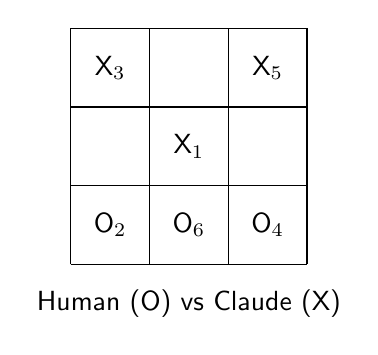
\begin{tikzpicture}
    % Draw grid
    \draw (0,0) grid (3,3);

    % Fill in moves
    \node at (0.5, 2.5) {X$_3$}; % Top-left
    \node at (2.5, 2.5) {X$_5$}; % Top-right
    \node at (1.5, 1.5) {X$_1$}; % Center
    
    \node at (0.5, 0.5) {O$_2$}; % Bottom-left
    \node at (1.5, 0.5) {O$_6$}; % Bottom-center
    \node at (2.5, 0.5) {O$_4$}; % Bottom-right

    % Labels
    \node at (1.5, -0.5) {Human (O) vs Claude (X)};
\end{tikzpicture}
\end{center}

Claude starts with a center move but fails to capitalize on it, leading to a loss. The model places Xs on the top corners but does not create a winning line and does not block the human's winning move.

\begin{center}
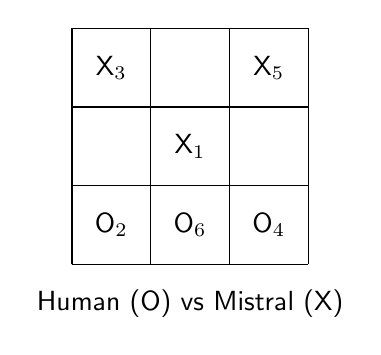
\begin{tikzpicture}
    % Draw grid
    \draw (0,0) grid (3,3);

    % Fill in moves
    \node at (0.5, 2.5) {X$_3$}; % Top-left
    \node at (2.5, 2.5) {X$_5$}; % Top-right
    \node at (1.5, 1.5) {X$_1$}; % Center
    
    \node at (0.5, 0.5) {O$_2$}; % Bottom-left
    \node at (1.5, 0.5) {O$_6$}; % Bottom-center
    \node at (2.5, 0.5) {O$_4$}; % Bottom-right

    % Labels
    \node at (1.5, -0.5) {Human (O) vs Mistral (X)};
\end{tikzpicture}
\end{center}

Mistral mirrors Claude’s strategy, starting in the center but failing to follow through effectively. The game ends in a loss too for the same reasons as above - a missed block.

\begin{center}
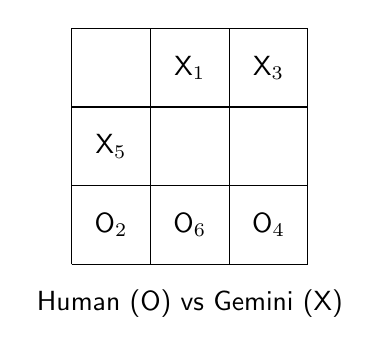
\begin{tikzpicture}
    % Draw grid
    \draw (0,0) grid (3,3);

    % Fill in moves
    \node at (1.5, 2.5) {X$_1$}; % Top-center
    \node at (2.5, 2.5) {X$_3$}; % Top-right
    \node at (0.5, 1.5) {X$_5$}; % Middle-left
    
    \node at (0.5, 0.5) {O$_2$}; % Bottom-left
    \node at (1.5, 0.5) {O$_6$}; % Bottom-center
    \node at (2.5, 0.5) {O$_4$}; % Bottom-right

    % Labels
    \node at (1.5, -0.5) {Human (O) vs Gemini (X)};
\end{tikzpicture}
\end{center}

Gemini deviates slightly by focusing on a top-row strategy but still fails to secure a win. The model also missed the blocking move.

All three models fail to block the winning move when they could clearly have done so.

Table \ref{table:other_models} shows the type of non-answers we obtained from a diverse set of models from Huggingface picked at random from the first 2 pages from the models listing page after sorting on most downloads. 

\begin{longtable}{p{4.5cm} p{9.5cm}} % Adjusted column widths for better alignment
\toprule
\textbf{Model Name} & \textbf{Model Answer} \\
\midrule
\endfirsthead

\toprule
\textbf{Model Name} & \textbf{Model Answer} \\
\midrule
\endhead

\midrule
\multicolumn{2}{r}{\textit{Continued on next page}} \\
\bottomrule
\endfoot

\bottomrule
\endlastfoot

microsoft/phi-2 \cite{phi2} & ``You will play as player 2, therefore you play with the symbol O while your adversary.'' \\
JackFram/llama-68m \cite{llama68m} & {+---+---+---+---+---+---+---+---+---+$\omega$ 1.} \\
openai-community/gpt2-medium \cite{gpt2medium} & ``The first player to guess correctly wins.'' \\
sshleifer/tiny-gpt2 \cite{tinygpt2} & ``LLM's turn to guess.'' factors factors factors factors factors factors factors factors factors factors factors factors factors factors factors factors factors factors factors. \\
TinyLlama/TinyLlama-1.1B-Chat-v1.0 \cite{tinyllama} & \texttt{def play\_tic\_tac\_toe():} \\
TinyLlama/TinyLlama-1.1B-Chat-v1.0 \cite{tinyllama} & \texttt{def play\_tic\_tac\_toe():} \\
mistralai/Mixtral-8x7B-Instruct-v0.1 \cite{mixtral} & Thank you for the instructions. I understand that we are playing a game of Tic-Tac-Toe, and I am player 1, using the mark 'X'. We will be taking turns entering our moves as row and column numbers. The game continues until one player wins by placing three of their marks in a horizontal, vertical, or diagonal row. Here's an example of how the input could look like for my first move: 0 1 This corresponds. \\
microsoft/DialoGPT-medium \cite{dialogptmedium} & It npmat, unless broken wall... \\
microsoft/Phi-3-mini-4k-instruct \cite{phi3} & Welcome to the Tic-Tac-Toe challenge! As player 1 with the mark X, you have the first turn. Here's a simple strategy you might use to begin the game: Place your X in the center square, which is row 1, column 1. Output: ``0 1''. By placing your X in the center, you maximize your chances of creating a winning combination, as the center square is a. \\
distilbert/distilgpt2 \cite{distilgpt2} & ``LLM's turn to guess.'' ``LLM's turn to guess.'' ``LLM's turn to guess.'' \\
openai-community/gpt2 \cite{gpt2} & ``The game is played on a 3x3 grid. Players take turns placing their mark.'' \\
Falcon-7B-Instruct \cite{falcon7b} & Here's a Python code that should work: \\
\label{table:other_models}
\end{longtable}

%%%  Please provide links to websites that provide 
%%%  further information relevant to the study 
%%%  (e.g., protocol download, troubleshooting 
%%%  forum, etc.). Clinical trial registry numbers 
%%%  and links should also be placed here. Please 
%%%  briefly describe the resource and its 
%%%  relevance for the paper. Please report this 
%%%  information as: “Description: URL.”

% Cell.com homepage: https://www.cell.com
% \newline Templates for Cell Press authors: https://www.cell.com/article-templates

%%%  ADDITIONAL MANUSCRIPT COMPONENTS:

%%%  Depending on the journal and the article 
%%%  type, you may be asked to upload the 
%%%  following as separate files: graphical 
%%%  abstract, highlights, eTOC blurb (In 
%%%  Brief), and/or other article components 
%%%  such as a "bigger picture" statement. 
%%%  These items are typically not required for 
%%%  initial submissions. Please refer to the 
%%%  journal's website, your acceptance 
%%%  letter, and/or the Final Files 
%%%  Requirements checklist to see if any of
%%%  these items are required (at any stage).


%\bibliography{main}
%\end{comment}

\end{document}